\newpage % Эта команда начинает новую страницу
\chapter{Введение в операционные системы}% Эта команда начинает первую лекцию. В фигурных скобках нужно
% записать тему лекции. Эта тема лекции автоматически получит порядковый номер и
% автоматически добавится в раздел <<Содержание>>. Лекций можно создавать сколько угодно.
% Для создания новой лекции скопируйте и вставьте (или наберите с клавиатуры) команду
% \chapter{Тема лекции} в любую часть рабочего файла. Можете смело менять местами лекции --
% вся нумерация после очередной компиляции поменяется автоматически.

% При необходимости здесь можно разместить любой текст
%-------------------------------------------------------------------------------------
%------------------------------СИСТЕМНОЕ ПО-------------------------------------------
%-------------------------------------------------------------------------------------

\section{Системное программное обеспечение}% Эта команда начнет раздел, который будем далее условно называть
% параграф. В роли параграфа будет выступать структурная часть лекции (отдельный раздел,
% вопрос и т.п.). В фигурных скобках нужно вписать название параграфа. Параграф автоматически
% получит порядковый номер, который будет состоять из двух чисел, разделенных точкой.
% Первое число -- порядковый номер лекции, второе число -- порядковый номер параграфа в
% пределах лекции. Параграфов можно создавать сколько угодно. Для создания нового параграфа
% скопируйте и вставьте (или наберите с клавиатуры) команду \section{Название параграфа} в
% любую часть рабочего файла. Можете смело менять местами параграфы, переносить их из одной
% лекции  в другую -- вся нумерация после очередной компиляции поменяется автоматически.

% При необходимости здесь можно разместить любой текст

\subsection{Структура программного обеспечения вычислительной системы}% Эта команда начинает подраздел, который далее будем
% условно называть подпараграфом. В фигурных скобках нужно вписать название подпараграфа.
% Подпараграф автоматически получит порядковый номер, который будет состоять из трех
% чисел, разделенных точками. Первое число -- порядковый номер лекции, второе число --
% порядковый номер параграфа, третье число -- порядковый номер подпараграфа. Подпараграфов
% можно создавать сколько угодно. Для создания нового подпараграфа скопируйте и вставьте
% (или наберите с клавиатуры) команду \subsection{Название подпараграфа} в любую часть
% Рабочего файла. Можете смело менять подпараграфы местами, переносить их из одного
% параграфа в другой (даже другой параграф другой лекции) -- вся нумерация после очередной
% компиляции поменяется автоматически.

Из чего состоит любая вычислительная система? Во-первых, из того, что в англоязычных странах принято называть словом hardware, или техническое обеспечение: процессор, память, монитор, дисковые устройства и т.д., объединенные магистральным соединением, которое называется шиной. Некоторые сведения об архитектуре компьютера имеются в приложении 1 к настоящей лекции.


Во-вторых, вычислительная система состоит из программного обеспечения. Все программное обеспечение принято делить на две части: прикладное и системное. К прикладному программному обеспечению, как правило, относятся разнообразные банковские и прочие бизнес-программы, игры, текстовые процессоры и т. п. Под системным программным обеспечением обычно понимают программы, способствующие функционированию и разработке прикладных программ. Надо сказать, что деление на прикладное и системное программное обеспечение является отчасти условным и зависит от того, кто осуществляет такое деление. Так, обычный пользователь, неискушенный в программировании, может считать Microsoft Word системной программой, а, с точки зрения программиста, это – приложение. Компилятор языка Си для обычного программиста – системная программа, а для системного – прикладная. Несмотря на эту нечеткую грань, данную ситуацию можно отобразить в виде последовательности слоев (см. рис. 1.1), выделив отдельно наиболее общую часть системного программного обеспечения – операционную систему:

\begin{figure}[h!]\center
   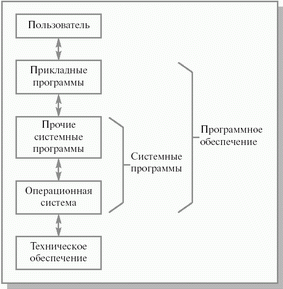
\includegraphics[scale=1.5]{pic1-1.png}
   \caption{Слои программного обеспечения компьютерной системы}\label{pic11}
\end{figure}

Схематично основные рассматриваемые здесь компоненты представлены на рис. 1.2.
В нижней части рисунка показано аппаратное обеспечение. Оно состоит из микросхем,
плат, дисков, клавиатуры, монитора и других физических объектов. Над аппаратным
обеспечением находится программное обеспечение. Большинство компьютеров имеют
два режима работы: режим ядра и режим пользователя.
Операционная система — наиболее фундаментальная часть программного обеспечения, работающая в режиме ядра (этот режим называют еще режимом супервизора). В этом режиме она имеет полный
доступ ко всему аппаратному обеспечению и может задействовать любую инструкцию,
которую машина в состоянии выполнить. Вся остальная часть программного обеспечения
работает в режиме пользователя, в котором доступно лишь подмножество инструкций
машины. В частности, программам, работающим в режиме пользователя, запрещено
использование инструкций, управляющих машиной или осуществляющих операции
ввода-вывода (Input/Output — I/O). К различиям между режимами ядра и пользователя
мы еще не раз вернемся на страницах этой книги. Эти различия оказывают решающее
влияние на порядок работы операционной системы.

\begin{figure}[h!]\center
   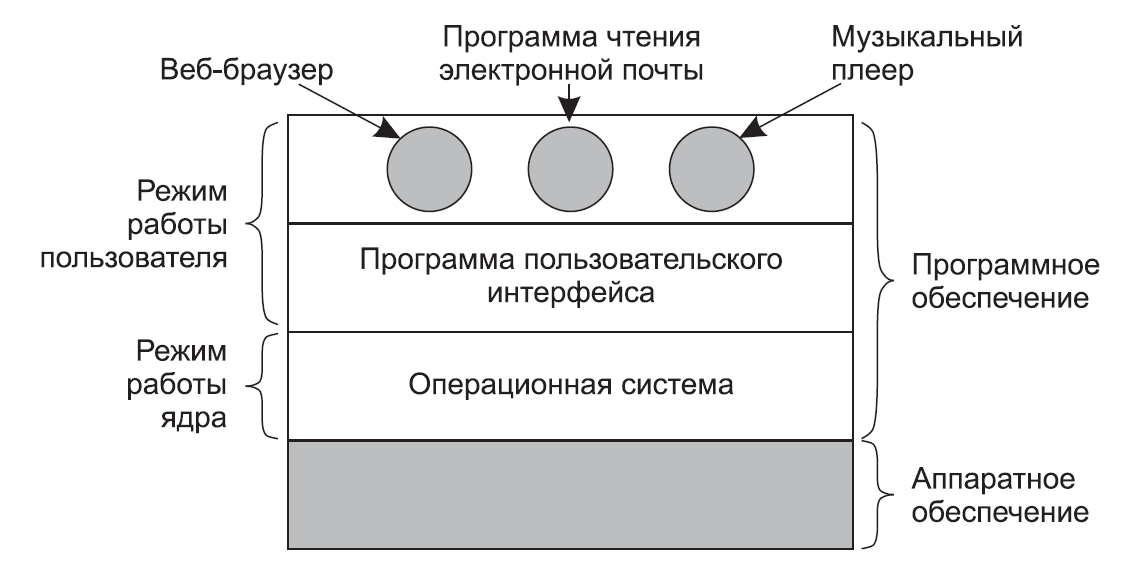
\includegraphics[scale=0.6]{pic1-2.png}
   \caption{Место операционной системы в структуре программного обеспечения}
\end{figure}

\newpage
%%---------------------------------------------------------------------------------
\subsection{Определение ОС}
Большинство пользователей имеет опыт эксплуатации операционных систем, но тем не менее они затруднятся дать этому понятию точное определение. Давайте кратко рассмотрим основные точки зрения.

\begin{opr}\rm \hypertarget{opr1_OS}{\textbf{Операционная система как виртуальная машина}
\end{opr}}
При разработке ОС широко применяется абстрагирование, которое является важным методом упрощения и позволяет сконцентрироваться на взаимодействии высокоуровневых компонентов системы, игнорируя детали их реализации. В этом смысле ОС представляет собой интерфейс между пользователем и компьютером.

Архитектура большинства компьютеров на уровне машинных команд очень неудобна для использования прикладными программами. Например, работа с диском предполагает знание внутреннего устройства его электронного компонента – контроллера для ввода команд вращения диска, поиска и форматирования дорожек, чтения и записи секторов и т. д. Ясно, что средний программист не в состоянии учитывать все особенности работы оборудования (в современной терминологии – заниматься разработкой драйверов устройств), а должен иметь простую высокоуровневую абстракцию, скажем представляя информационное пространство диска как набор файлов. Файл можно открывать для чтения или записи, использовать для получения или сброса информации, а потом закрывать. Это концептуально проще, чем заботиться о деталях перемещения головок дисков или организации работы мотора. Аналогичным образом, с помощью простых и ясных абстракций, скрываются от программиста все ненужные подробности организации прерываний, работы таймера, управления памятью и т. д. Более того, на современных вычислительных комплексах можно создать иллюзию неограниченного размера оперативной памяти и числа процессоров. Всем этим занимается операционная система. Таким образом, операционная система представляется пользователю виртуальной машиной, с которой проще иметь дело, чем непосредственно с оборудованием компьютера.

\begin{opr}\rm \hypertarget{opr2_OS}{\textbf{Операционная система как менеджер ресурсов}
\end{opr}}
Операционная система предназначена для управления всеми частями весьма сложной архитектуры компьютера. Представим, к примеру, что произойдет, если несколько программ, работающих на одном компьютере, будут пытаться одновременно осуществлять вывод на принтер. Мы получили бы мешанину строчек и страниц, выведенных различными программами. Операционная система предотвращает такого рода хаос за счет буферизации информации, предназначенной для печати, на диске и организации очереди на печать. Для многопользовательских компьютеров необходимость управления ресурсами и их защиты еще более очевидна. Следовательно, операционная система, как менеджер ресурсов, осуществляет упорядоченное и контролируемое распределение процессоров, памяти и других ресурсов между различными программами.
Современные операционные системы допускают одновременную работу нескольких
программ.Когда с компьютером (или с сетью) работают несколько пользователей, потребности в управлении и защите памяти, устройств ввода-вывода и других ресурсов значительно возрастают, поскольку иначе пользователи будут мешать друг другу работать. Кроме этого, пользователям часто требуется совместно использовать не только аппаратное обеспечение, но и информацию (файлы, базы данных и т. п.).
Управление ресурсами включает в себя \textbf{мультиплексирование} (распределение) ресурсов двумя различными способами: во времени и в пространстве. Когда ресурс разделяется во времени, различные программы или пользователи используют его по очереди: сначала ресурс получают в пользование одни, потом другие и т. д. К примеру, располагая лишь одним центральным процессором и несколькими программами, стремящимися на нем выполняться, операционная система сначала выделяет центральный процессор одной программе, затем, после того как она уже достаточно поработала, центральный процессор получает в свое распоряжение другая программа, затем еще одна программа, и, наконец, его опять получает в свое распоряжение первая программа. Определение того, как именно ресурс будет разделяться во времени — кто будет следующим потребителем и как долго, — это задача операционной системы. Другим примером мультиплексирования во времени может послужить совместное использование принтера. Когда в очереди для распечатки на одном принтере находятся несколько заданий на печать, нужно принять решение, какое из них будет выполнено следующим.
Другим видом разделения ресурсов является пространственное разделение. Вместо поочередной работы каждый клиент получает какую-то часть разделяемого ресурса. Например, оперативная память обычно делится среди нескольких работающих программ, так что все они одновременно могут постоянно находиться в памяти (например, используя центральный процессор по очереди). При условии, что памяти достаточно для хранения более чем одной программы, эффективнее разместить в памяти сразу несколько программ, чем выделять всю память одной программе, особенно если ей нужна лишь небольшая часть от общего пространства. Разумеется, при этом возникают проблемы равной доступности, обеспечения безопасности и т. д., и их должна решать операционная система. Другим ресурсом с разделяемым пространством является жесткий диск. На многих системах на одном и том же диске могут одновременно храниться файлы, принадлежащие многим пользователям. Распределение дискового пространства и отслеживание того, кто какие дисковые блоки использует, — это типичная задача операционной системы по управлению ресурсами.

\begin{opr}\rm \hypertarget{opr3_OS}{\textbf{Операционная система как защитник пользователей и программ}}
\end{opr}
Если вычислительная система допускает совместную работу нескольких пользователей, то возникает проблема организации их безопасной деятельности. Необходимо обеспечить сохранность информации на диске, чтобы никто не мог удалить или повредить чужие файлы. Нельзя разрешить программам одних пользователей произвольно вмешиваться в работу программ других пользователей. Нужно пресекать попытки несанкционированного использования вычислительной системы. Всю эту деятельность осуществляет операционная система как организатор безопасной работы пользователей и их программ. С такой точки зрения операционная система представляется системой безопасности государства, на которую возложены полицейские и контрразведывательные функции.

\begin{opr}\rm \hypertarget{opr4_OS}{\textbf{Операционная система как постоянно функционирующее ядро}}
\end{opr}
Наконец, можно дать и такое определение: операционная система – это программа, постоянно работающая на компьютере и взаимодействующая со всеми прикладными программами. Казалось бы, это абсолютно правильное определение, но, как мы увидим дальше, во многих современных операционных системах постоянно работает на компьютере лишь часть операционной системы, которую принято называть ее ядром.

Как мы видим, существует много точек зрения на то, что такое операционная система. Невозможно дать ей адекватное строгое определение. Нам проще сказать не что есть операционная система, а для чего она нужна и что она делает. Для выяснения этого вопроса рассмотрим историю развития вычислительных систем.
\newline

Как мы видим, существует много точек зрения на то, что такое операционная система. Невозможно дать ей адекватное строгое определение. Нам проще сказать не что есть операционная система, а для чего она нужна и что она делает:
%%itemize - маркированный список
\begin{itemize}
   \item {\hyperlink{opr1_OS}{ОС как виртуальная машина}}
   \item {\hyperlink{opr2_OS}{ОС как менеджер ресурсов}}
   \item {\hyperlink{opr3_OS}{ОС как защитник пользователей и программ}}
   \item {\hyperlink{opr4_OS}{ОС как постоянно функционирующее ядро}}
\end{itemize}
\newpage
%%---------------------------------------------------------------------------------
\subsection{Требования, предъявляемые к ОС}
Операционная система является сердцевиной сетевого программного обеспечения, она создает среду для выполнения приложений и во многом определяет, какими полезными для пользователя свойствами эти приложения будут обладать. В связи с этим рассмотрим требования, которым должна удовлетворять современная ОС.

Очевидно, что главным требованием, предъявляемым к операционной системе, является способность выполнения основных функций: эффективного управления ресурсами и обеспечения удобного интерфейса для пользователя и прикладных программ. Современная ОС, как правило, должна реализовывать мультипрограммную обработку, виртуальную память, свопинг, поддерживать многооконный интерфейс, а также выполнять многие другие, совершенно необходимые функции. Кроме этих функциональных требований к операционным системам предъявляются не менее важные рыночные требования. К этим требованиям относятся:
\begin{itemize}
   \item \hyperlink{opr1_REQ}{\textit{Расширяемость}}

         Код должен быть написан таким образом, чтобы можно было легко внести дополнения и изменения, если это потребуется, и не нарушить целостность системы.
   \item \hyperlink{opr2_REQ}{\textit{Переносимость}}

         Код должен легко переноситься с процессора одного типа на процессор другого типа и с аппаратной платформы (которая включает наряду с типом процессора и способ организации всей аппаратуры компьютера) одного типа на аппаратную платформу другого типа.
   \item \textit{Надежность и отказоустойчивость}

         Система должна быть защищена как от внутренних, так и от внешних ошибок, сбоев и отказов. Ее действия должны быть всегда предсказуемыми, а приложения не должны быть в состоянии наносить вред ОС.
   \item \hyperlink{opr3_REQ}{\textit{Совместимость}}

         ОС должна иметь средства для выполнения прикладных программ, написанных для других операционных систем. Кроме того, пользовательский интерфейс должен быть совместим с существующими системами и стандартами.
   \item \hyperlink{opr4_REQ}{\textit{Безопасность}}

         ОС должна обладать средствами защиты ресурсов одних пользователей от других.
   \item \textit{Производительность}

         Система должна обладать настолько хорошим быстродействием и временем реакции, насколько это позволяет аппаратная платформа.
\end{itemize}

\hypertarget{opr1_REQ}{\textbf{Расширяемость}}

В то время, как аппаратная часть компьютера устаревает за несколько лет, полезная жизнь операционных систем может измеряться десятилетиями. Примером может служить ОС UNIX. Поэтому операционные системы всегда эволюционно изменяются со временем, и эти изменения более значимы, чем изменения аппаратных средств. Изменения ОС обычно представляют собой приобретение ею новых свойств. Например, поддержка новых устройств, таких как CD-ROM, возможность связи с сетями нового типа, поддержка многообещающих технологий, таких как графический интерфейс пользователя или объектно-ориентированное программное окружение, использование более чем одного
процессора. Сохранение целостности кода, какие бы изменения не вносились в операционную систему, является главной целью разработки.

Расширяемость может достигаться за счет модульной структуры ОС, при которой программы строятся из набора отдельных модулей, взаимодействующих только через функциональный интерфейс. Новые компоненты могут быть добавлены в операционную систему модульным путем, они выполняют свою работу, используя интерфейсы, поддерживаемые существующими компонентами.

Использование объектов для представления системных ресурсов также улучшает расширяемость системы. Объекты - это абстрактные типы данных, над которыми можно производить только те действия, которые предусмотрены специальным набором объектных функций. Объекты позволяют единообразно управлять системными ресурсами. Добавление новых объектов не разрушает существующие объекты и не требует изменений существующего кода.

Прекрасные возможности для расширения предоставляет подход к структурированию ОС по типу клиент-сервер с использованием микроядерной технологии. В соответствии с этим подходом ОС строится как совокупность привилегированной управляющей программы и набора непривилегированных услуг-серверов. Основная часть ОС может оставаться неизменной в то время, как могут быть добавлены новые серверы или улучшены старые.
Средства вызова удаленных процедур (RPC) также дают возможность расширить функциональные возможности ОС. Новые программные процедуры могут быть добавлены в любую машину сети и немедленно поступить в распоряжение прикладных программ на других машинах сети.

Некоторые ОС для улучшения расширяемости поддерживают загружаемые драйверы, которые могут быть добавлены в систему во время ее работы. Новые файловые системы, устройства и сети могут поддерживаться путем написания драйвера устройства, драйвера файловой системы или транспортного драйвера и загрузки его в систему.
\newline

\hypertarget{opr2_REQ}{\textbf{Переносимость}}

Требование переносимости кода тесно связано с расширяемостью. Расширяемость позволяет улучшать операционную систему, в то время как переносимость дает возможность перемещать всю систему на машину, базирующуюся на другом процессоре или аппаратной платформе, делая при этом по возможности небольшие изменения в коде. Хотя ОС часто описываются либо как переносимые, либо как непереносимые, переносимость - это не бинарное состояние. Вопрос не в том, может ли быть система перенесена, а в том, насколько легко можно это сделать. Написание переносимой ОС аналогично написанию любого переносимого кода - нужно следовать некоторым правилам.

Во-первых, большая часть кода должна быть написана на языке, который имеется на всех машинах, куда вы хотите переносить систему. Обычно это означает, что код должен быть написан на языке высокого уровня, предпочтительно стандартизованном, например, на языке С. Программа, написанная на ассемблере, не является переносимой, если только вы не собираетесь переносить ее на машину, обладающую командной совместимостью с вашей.
Во-вторых, следует учесть, в какое физическое окружение программа должна быть перенесена. Различная аппаратура требует различных решений при создании ОС. Например, ОС, построенная на 32-битовых адресах, не может быть перенесена на машину с 16-битовыми адресами (разве что с огромными трудностями).

В-третьих, важно минимизировать или, если возможно, исключить те части кода, которые непосредственно взаимодействуют с аппаратными средствами. Зависимость от аппаратуры может иметь много форм. Некоторые очевидные формы зависимости включают прямое манипулирование регистрами и другими аппаратными средствами.

В-четвертых, если аппаратно зависимый код не может быть полностью исключен, то он должен быть изолирован в нескольких хорошо локализуемых модулях. Аппаратно-зависимый код не должен быть распределен по всей системе. Например, можно спрятать аппаратно-зависимую структуру в программно-задаваемые данные абстрактного типа. Другие модули системы будут работать с этими данными, а не с аппаратурой, используя набор некоторых функций. Когда ОС переносится, то изменяются только эти данные и функции, которые ими манипулируют.

Для легкого переноса ОС при ее разработке должны быть соблюдены следующие требования:
\begin{enumerate}
   \item Переносимый язык высокого уровня.

         Большинство переносимых ОС написано на языке С (стандарт ANSI X3.159-1989). Разработчики выбирают С потому, что он стандартизован, и потому, что С-компиляторы широко доступны. Ассемблер используется только для тех частей системы, которые должны непосредственно взаимодействовать с аппаратурой (например, обработчик прерываний) или для частей, которые требуют максимальной скорости (например, целочисленная арифметика повышенной точности). Однако непереносимый код должен быть тщательно изолирован внутри тех компонентов, где он используется.
   \item Изоляция процессора.

         Некоторые низкоуровневые части ОС должны иметь доступ к процессорно-зависимым структурам данных и регистрам. Однако код, который делает это, должен содержаться в небольших модулях, которые могут быть заменены аналогичными модулями для других процессоров.
   \item Изоляция платформы.

         Зависимость от платформы заключается в различиях между рабочими станциями разных производителей, построенными на одном и том же процессоре (например, MIPS R4000). Должен быть введен программный уровень, абстрагирующий аппаратуру (кэши, контроллеры прерываний ввода-вывода и т. п.) вместе со слоем низкоуровневых программ таким образом, чтобы высокоуровневый код не нуждался в изменении при переносе с одной платформы на другую.
\end{enumerate}


\hypertarget{opr3_REQ}{\textbf{Совместимость}}


Одним из аспектов совместимости является способность ОС выполнять программы, написанные для других ОС или для более ранних версий данной операционной системы, а также для другой аппаратной платформы.

Необходимо разделять вопросы двоичной совместимости и совместимости на уровне исходных текстов приложений. Двоичная совместимость достигается в том случае, когда можно взять исполняемую программу и запустить ее на выполнение на другой ОС. Для этого необходимы: совместимость на уровне команд процессора, совместимость на уровне системных вызовов и даже на уровне библиотечных вызовов, если они являются динамически связываемыми.

Совместимость на уровне исходных текстов требует наличия соответствующего компилятора в составе программного обеспечения, а также совместимости на уровне библиотек и системных вызовов. При этом необходима перекомпиляция имеющихся исходных текстов в новый выполняемый модуль.

Совместимость на уровне исходных текстов важна в основном для разработчиков приложений, в распоряжении которых эти исходные тексты всегда имеются. Но для
конечных пользователей практическое значение имеет только двоичная совместимость, так как только в этом случае они могут использовать один и тот же коммерческий продукт, поставляемый в виде двоичного исполняемого кода, в различных операционных средах и на различных машинах.

Обладает ли новая ОС двоичной совместимостью или совместимостью исходных текстов с существующими системами, зависит от многих факторов. Самый главный из них - архитектура процессора, на котором работает новая ОС. Если процессор, на который переносится ОС, использует тот же набор команд (возможно с некоторыми добавлениями) и тот же диапазон адресов, тогда двоичная совместимость может быть достигнута достаточно просто.

Гораздо сложнее достичь двоичной совместимости между процессорами, основанными на разных архитектурах. Для того, чтобы один компьютер выполнял программы другого (например, DOS-программу на Mac), этот компьютер должен работать с машинными командами, которые ему изначально непонятны. Например, процессор типа 680x0 на Mac должен исполнять двоичный код, предназначенный для процессора 80x86 в PC. Процессор 80x86 имеет свои собственные дешифратор команд, регистры и внутреннюю архитектуру. Процессор 680x0 не понимает двоичный код 80x86, поэтому он должен выбрать каждую команду, декодировать ее, чтобы определить, для чего она предназначена, а затем выполнить эквивалентную подпрограмму, написанную для 680x0. Так как к тому же у 680x0 нет в точности таких же регистров, флагов и внутреннего арифметико-логического устройства, как в 80x86, он должен имитировать все эти элементы с использованием своих регистров или памяти. И он должен тщательно воспроизводить результаты каждой команды, что требует специально написанных подпрограмм для 680x0, гарантирующих, что состояние эмулируемых регистров и флагов после выполнения каждой команды будет в точности таким же, как и на реальном 80x86.

Это простая, но очень медленная работа, так как микрокод внутри процессора 80x86 исполняется на значительно более быстродействующем уровне, чем эмулирующие его внешние команды 680x0. За время выполнения одной команды 80x86 на 680x0, реальный 80x86 может выполнить десятки команд. Следовательно, если процессор, производящий эмуляцию, не настолько быстр, чтобы компенсировать все потери при эмуляции, то программы, исполняющиеся под эмуляцией, будут очень медленными.

Выходом в таких случаях является использование так называемых прикладных сред. Учитывая, что основную часть программы, как правило, составляют вызовы библиотечных функций, прикладная среда имитирует библиотечные функции целиком, используя заранее написанную библиотеку функций аналогичного назначения, а остальные команды эмулирует каждую по отдельности.

Соответствие стандартам POSIX также является средством обеспечения совместимости программных и пользовательских интерфейсов. Во второй половине 80-х правительственные агентства США начали разрабатывать POSIX как стандарты на поставляемое оборудование при заключении правительственных контрактов в компьютерной области. POSIX - это "интерфейс переносимой ОС, базирующейся на UNIX". POSIX - собрание международных стандартов интерфейсов ОС в стиле UNIX. Использование стандарта POSIX (IEEE стандарт 1003.1 - 1988) позволяет создавать программы стиле UNIX, которые могут легко переноситься из одной системы в другую.
\newline

\hypertarget{opr4_REQ}{\textbf{Безопасность}}

В дополнение к стандарту POSIX правительство США также определило требования компьютерной безопасности для приложений, используемых правительством. Многие из этих требований являются желаемыми свойствами для любой многопользовательской системы. Правила безопасности определяют такие свойства, как защита ресурсов одного пользователя от других и установление квот по ресурсам для предотвращения захвата одним пользователем всех системных ресурсов ( таких как память).

Обеспечение защиты информации от несанкционированного доступа является обязательной функцией сетевых операционных систем. В большинстве популярных систем гарантируется степень безопасности данных, соответствующая уровню С2 в системе стандартов США.
Основы стандартов в области безопасности были заложены "Критериями оценки надежных компьютерных систем". Этот документ, изданный в США в 1983 году национальным центром компьютерной безопасности (NCSC - National Computer Security Center), часто называют Оранжевой Книгой.

В соответствии с требованиями Оранжевой книги безопасной считается такая система, которая "посредством специальных механизмов защиты контролирует доступ к информации таким образом, что только имеющие соответствующие полномочия лица или процессы, выполняющиеся от их имени, могут получить доступ на чтение, запись, создание или удаление информации".
\newpage
Иерархия уровней безопасности, приведенная в Оранжевой Книге, помечает низший уровень безопасности как D, а высший - как А.
\begin{enumerate}
   \item В класс D попадают системы, оценка которых выявила их несоответствие требованиям всех других классов.
   \item Основными свойствами, характерными для С-систем, являются: наличие подсистемы учета событий, связанных с безопасностью, и избирательный контроль доступа. Уровень С делится на 2 подуровня: уровень С1, обеспечивающий защиту данных от ошибок пользователей, но не от действий злоумышленников, и более строгий уровень С2. На уровне С2 должны присутствовать средства секретного входа, обеспечивающие идентификацию пользователей путем ввода уникального имени и пароля перед тем, как им будет разрешен доступ к системе. Избирательный контроль доступа, требуемый на этом уровне позволяет владельцу ресурса определить, кто имеет доступ к ресурсу и что он может с ним делать. Владелец делает это путем предоставляемых прав доступа пользователю или группе пользователей. Средства учета и наблюдения (auditing) - обеспечивают возможность обнаружить и зафиксировать важные события, связанные с безопасностью, или любые попытки создать, получить доступ или удалить системные ресурсы. Защита памяти - заключается в том, что память инициализируется перед тем, как повторно используется. На этом уровне система не защищена от ошибок пользователя, но поведение его может быть проконтролировано по записям в журнале, оставленным средствами наблюдения и аудитинга.
   \item Системы уровня В основаны на помеченных данных и распределении пользователей по категориям, то есть реализуют мандатный контроль доступа. Каждому пользователю присваивается рейтинг защиты, и он может получать доступ к данным только в соответствии с этим рейтингом. Этот уровень в отличие от уровня С защищает систему от ошибочного поведения пользователя.
   \item Уровень А является самым высоким уровнем безопасности, он требует в дополнение ко всем требованиям уровня В выполнения формального, математически обоснованного доказательства соответствия системы требованиям безопасности.

\end{enumerate}

Различные коммерческие структуры (например, банки) особо выделяют необходимость учетной службы, аналогичной той, что предлагают государственные рекомендации С2. Любая деятельность, связанная с безопасностью, может быть отслежена и тем самым учтена. Это как раз то, что требует С2 и то, что обычно нужно банкам. Однако, коммерческие пользователи, как правило, не хотят расплачиваться производительностью за повышенный уровень безопасности. А-уровень безопасности занимает своими управляющими механизмами до 90\% процессорного времени. Более безопасные системы не только снижают эффективность, но и существенно ограничивают число доступных прикладных пакетов, которые соответствующим образом могут выполняться в подобной системе. Например для ОС Solaris (версия UNIX) есть несколько тысяч приложений, а для ее аналога В-уровня - только сотня.
%%---------------------------------------------------------------------------------
\subsection{Основные принципы построения ОС}
\textbf{Частотный принцип}

Это наиболее общий принцип реализации системных программ. Основан на выделении в алгоритмах в обрабатывающих массивах действий данных по частоте использования. Для наиболее частых создаются условия быстрого выполнения. Например такие программы или данные хранятся в ОЗУ. Кроме того стараются оптимизировать код частых операций.
\newline

\textbf{Принцип модульности}

Отражая технологические и эксплуатационны6е свойства он наиболее эффективен, когда распространяется на ОС, прикладные программы и аппаратуру. Под модулем понимают функциональный элемент системы, законченный и выполненный в ее рамках и средства сопряжения с подобными элементами этой или другой системы. Для сопряжения используется интерфейс.

\begin{opr}\textit{Интерфейс} – система унифицированных связей и сигналов для взаимодействия частей ВС. При наличии заданного интерфейса модуль можно легко заменить на другой. Деление на модули происходит по функциональному признаку. Есть 2 способа проектирования:
\end{opr}
\begin{enumerate}
   \item Нисходящее – от общего к частному.
         Дробление осуществляется до отдельных транслируемых единиц. Модули строят с учетом их использования в будущем.
   \item Восходящий метод. Составляют из существующих функциональных модулей более крупные.
\end{enumerate}

Иерархически упрощенна структура значительно упрощает разработку, уменьшает число ошибок, повышает надежность при эксплуатации.
Если модуль в процессе работы изменяет себя так, что повторное его исполнение невозможно – это однократный модуль. Если он себя не меняет или изменив восстанавливает – многократные модуль. Бывает случай, когда в многозадачных средах для исключения дублирования многократными модулями пользуются разные пользователи. Если модуль может обслуживать несколько заявок одновременно (первая еще не завершена, а вторую уже начали обслуживать), то такой модуль называется реентерабельным. Это достигается разными способами (усилиям программиста).
\newline

\textbf{Принцип функциональной избирательности}

Это сочетание 2-х типов. В ОС выделяется некоторая часть постоянных модулей, которые постоянно должны быть под рукой. Они составляют ядро ОС.

Инженерная задача – выбор решения при наличии противоречивых требований, основанных на оптимальном компромиссе. При формировании ядра возникает инженерная задача. В состав должны входить наиболее часто используемые модули, но с другой стороны количество занимаемой памяти не должно быть слишком большим. Поэтому, как правило, в ядро входят модули по управлению системой прерываний, диспетчеры памяти и времени ЦП и некоторые части планировщика. Как правило они постоянно находятся в ОЗУ- резиденты. Кроме них существуют транзитные модули, которые находятся на магнитных дисках, внешних устройствах и загружаются в ОЗУ по сере их необходимости, иногда перекрывая друг друга.
\newline

\textbf{Принцип генерируемости}

ОС должна быть настроена на конфигурацию конкретной ВС. Это происходит редко. Источником ОС является дистрибутивный том, транспортная магнитная лента и т.д. Это может быть простое копирование нужных модулей на системный ток (такая технология используется в ДОС) или использование специальной программы со своим входным языком. В результате генерации получается полная версия ОС, адаптированная к конкретной конфигурации ВС и запросам пользователей. Модульность упрощает генерацию.
\newline

\textbf{Принцип функциональной избыточности}

Это возможность выполнения одной и той же работы несколькими способами. Это надо для повышения надежности. Пример: Для ОС ЕС для пакетной обработки допускается при конфигурации: MFT, MVT, SVS. B RT-11 используется 5 видов мониторов а монитор – это управляющая программа ОС. В ОС DVCПАК существует 2 способа запуска задачи на чсет: пакетный режим и режим подчиненной задачи. В DOS вывести файл - type или copy…con
\newline

\textbf{Принцип по умолчанию}

Заключается в облегчении взаимодействия в системах при генерации и при работе. Его смысл основан на хранении в системе некоторых базовых описаний и характеристик. Определяющих прогнозируемые параметры, объем ОЗУ, время счета и т.д. Эту информацию ОС использует, если пользователь или оператор забудет или умышленно не конкретизирует. Число и значение этих параметров могут определятся при генерации или старте ОС и некоторые из них могут динамически изменяться в процессе работы.
\newline

\textbf{Принцип перемещаемости}

Смысл: работоспособность модулей не зависит от их расположения в ОЗУ, т. к. разные модули могут в разных случаях загружаться по разным адресам. Для этого их пишут в перемещаемом коде либо выполняют настройку адресов во время загрузки. Это необходимо, т.к. неизвестно куда будет загружаться модуль в очередной раз, по какому адресу. Этим свойством могут обладать и прикладные программы.
\newline

\textbf{Принцип защиты}

Его смысл в ограждении программ и данных пользователя от искажений и нежелательных взаимных влияний. Данные должны защищаться и при хранении и при выполнении. При работе обычно используется аппаратная защита – включение в код программ привилегированных программ (команд), которые недоступны в режиме пользователя, но доступны ОС.
Один из эффективных способов – контекстная защита, которая основана на известности исполнительного адреса: если адрес не принадлежит контексту задачи, происходит программное прерывание – это аппаратная защита.

Наиболее распространены граничные регистры и защита по ключу.

Традиционным способом защиты является защита при помощи пароля. При правильно выбранном пароле он (способ) является простым и эффективным.

Пример: в Windows 95 ресурс в зависимости от пароля может быть доступен для чтения или чтения/записи. В UNIX 3 вида прав: Чтение, Запись, Выполнение.
\newline

\textbf{Принцип независимости программ от внешних устройств}

Желательно, что бы программы пользователя работали со внешними устройствами однотипно, независимо от их физических характеристик. Связь программ с физическими устройствами осуществляется не при трансляции, а при выполнении.

Достоинства:
Можно реализовать практически одинаковый интерфейс взаимодействия с пользовательской программой для всех устройств.

Код обслуживания устройств не дублируется в пользовательских программах.
Обычно код обслуживания ПУ оформляется в виде отдельных модулей (драйверов). В зависимости от ОС драйверы могут грузиться при старте ОС, либо в процессе работы. Наиболее последовательно этот принцип реализован в UNIX.
\newline

\textbf{Принцип открытости и наращиваемости}

ОТКРЫТОСТЬ - подразумевает доступность ОС для анализа и использования.
Пример: DOS – открытая, т. к. описан интерфейс взаимодействия с ней.
Наращиваемость позволяет вводить в ОС новые модули. Это возможно если ОС открыта.

%------------------------------------------------------------------------------------
\newpage
%-------------------------------------------------------------------------------------
%------------------------------КЛАССИФИКАЦИЯ ОС---------------------------------------
%-------------------------------------------------------------------------------------

\section{Классификация ОС}
%------------------------------------------------------------------------------------
\subsection{Этапы развития ОС}

\textbf{Первый период (1945 -1955). Ламповые машины. Операционных систем нет}

Известно, что компьютер был изобретен английским математиком Чарльзом Бэбиджем в конце восемнадцатого века. Его "аналитическая машина" так и не смогла но-настоящему заработать, потому что технологии того времени не удовлетворяли требованиям по изготовлению деталей точной механики, которые были необходимы для вычислительной техники. Известно также, что этот компьютер не имел операционной системы.

Опуская историю механических и электромеханических устройств перейдём сразу к цифровым. Некоторый прогресс в создании цифровых вычислительных машин произошел после второй мировой войны. В середине 40-х были созданы первые ламповые вычислительные устройства и появился принцип программы, хранящейся в памяти машины (John Von Neumann, июнь 1945 г.).. В то время одна и та же группа людей участвовала и в проектировании, и в эксплуатации, и в программировании вычислительной машины. Это была скорее научно-исследовательская работа в области вычислительной техники, а не использование компьютеров в качестве инструмента решения каких-либо практических задач из других прикладных областей. Программирование осуществлялось исключительно на машинном языке. Об операционных системах не было и речи, все задачи организации вычислительного процесса решались вручную каждым программистом с пульта управления.

Программа загружалась в память машины в лучшем случае с колоды перфокарт, а обычно с помощью панели переключателей.

Вычислительная система выполняла одновременно только одну операцию (ввод-вывод или собственно вычисления). Отладка программ велась с пульта управления с помощью изучения состояния памяти и регистров машины. В конце этого периода появляется первое системное программное обеспечение: в 1951–1952 гг. возникают прообразы первых компиляторов с символических языков (Fortran и др.), а в 1954 г. Nat Rochester разрабатывает Ассемблер для IBM-701. Другого системного программного обеспечения, кроме библиотек математических и служебных подпрограмм, не было.

Существенная часть времени уходила на подготовку запуска программы, а сами программы выполнялись строго последовательно. Такой режим работы называется \textit{последовательной обработкой данных}. В целом первый период характеризуется крайне высокой стоимостью вычислительных систем, их малым количеством и низкой эффективностью использования.

\textbf{Второй период (1955 - 1965). Компьютеры на основе транзисторов. Пакетные операционные системы}

С середины 50-х годов начался следующий период в эволюции вычислительной техники, связанный с появлением новой технической базы – полупроводниковых элементов. Применение транзисторов вместо часто перегоравших электронных ламп привело к повышению надежности компьютеров. Теперь машины могут непрерывно работать достаточно долго, чтобы на них можно было возложить выполнение практически важных задач. Снижается потребление вычислительными машинами электроэнергии, совершенствуются системы охлаждения. Размеры компьютеров уменьшились. Снизилась стоимость эксплуатации и обслуживания вычислительной техники. Началось использование ЭВМ коммерческими фирмами. Одновременно наблюдается бурное развитие алгоритмических языков (LISP, COBOL, ALGOL-60, PL-1 и т.д.). Появляются первые настоящие компиляторы, редакторы связей, библиотеки математических и служебных подпрограмм. Упрощается процесс программирования. Пропадает необходимость взваливать на одних и тех же людей весь процесс разработки и использования компьютеров. Именно в этот период происходит разделение персонала на программистов и операторов, специалистов по эксплуатации и разработчиков вычислительных машин.

Изменяется сам процесс прогона программ. Теперь пользователь приносит программу с входными данными в виде колоды перфокарт и указывает необходимые ресурсы. Такая колода получает название задания. Оператор загружает задание в память машины и запускает его на исполнение. Полученные выходные данные печатаются на принтере, и пользователь получает их обратно через некоторое (довольно продолжительное) время.
\begin{figure}\center
   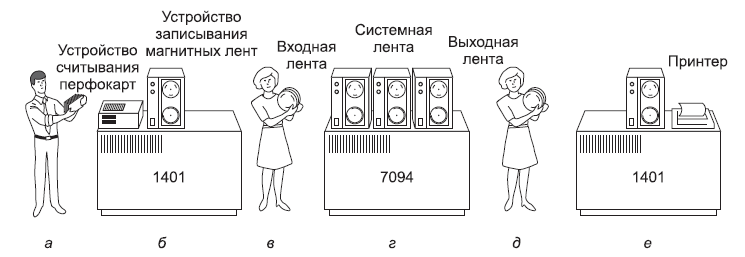
\includegraphics[scale=1]{pic2-1.png}
   \caption{Ранняя система пакетной обработки: а — программист приносит карты для IBM 1401; б — IBM 1401 записывает пакет заданий на магнитную ленту; в — оператор переносит входные данные на ленте к IBM 7094; г — IBM 7094 выполняет вычисления; д — оператор переносит ленту с выходными данными на IBM 1401; е — IBM 1401 печатает выходные данные}
\end{figure}

Смена запрошенных ресурсов вызывает приостановку выполнения программ, в результате процессор часто простаивает. Для повышения эффективности использования компьютера задания с похожими ресурсами начинают собирать вместе, создавая пакет заданий.

Появляются первые системы пакетной обработки, которые просто автоматизируют запуск одной программы из пакета за другой и тем самым увеличивают коэффициент загрузки процессора. При реализации систем пакетной обработки был разработан формализованный язык управления заданиями, с помощью которого программист сообщал системе и оператору, какую работу он хочет выполнить на вычислительной машине. Системы пакетной обработки стали прообразом современных операционных систем, они были первыми системными программами, предназначенными для управления вычислительным процессом.

\textbf{Третий период (1965 - 1980). Компьютеры на основе интегральных микросхем.Первые многозадачные ОС}

Следующий важный период развития вычислительных машин относится к 1965-1980 годам. В это время в технической базе произошел переход от отдельных полупроводниковых элементов типа транзисторов к интегральным микросхемам, что дало гораздо большие возможности новому, третьему поколению компьютеров.

Для этого периода характерно также создание семейств программно-совместимых машин. Первым семейством программно-совместимых машин, построенных на интегральных микросхемах, явилась серия машин IBM/360. Построенное в начале 60-х годов это семейство значительно превосходило машины второго поколения по критерию цена/производительность. Вскоре идея программно-совместимых машин стала общепризнанной.
Программная совместимость требовала и совместимости операционных систем. Такие операционные системы должны были бы работать и на больших, и на малых вычислительных системах, с большим и с малым количеством разнообразной периферии, в коммерческой области и в области научных исследований. Операционные системы, построенные с намерением удовлетворить всем этим противоречивым требованиям, оказались чрезвычайно сложными "монстрами". Они состояли из многих миллионов ассемблерных строк, написанных тысячами программистов, и содержали тысячи ошибок, вызывающих нескончаемый поток исправлений. В каждой новой версии операционной системы исправлялись одни ошибки и вносились другие.

Однако, несмотря на необозримые размеры и множество проблем, OS/360 и другие ей подобные операционные системы машин третьего поколения действительно удовлетворяли большинству требований потребителей. Важнейшим достижением ОС данного поколения явилась реализация мультипрограммирования.
\begin{opr}
   Мультипрограммирование- это способ организации вычислительного процесса, при котором на одном процессоре попеременно выполняются несколько программ.
\end{opr} Пока одна программа выполняет операцию ввода-вывода, процессор не простаивает, как это происходило при последовательном выполнении программ (однопрограммный режим), а выполняет другую программу (многопрограммный режим). При этом каждая программа загружается в свой участок оперативной памяти, называемый разделом.

\begin{figure}\center
   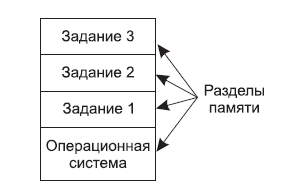
\includegraphics[scale=1.3]{pic2-2.png}
   \caption{Многозадачная система с тремя заданиями в памяти}
\end{figure}

Другое нововведение - спулинг (spooling). Спулинг в то время определялся как способ организации вычислительного процесса, в соответствии с которым задания считывались с перфокарт на диск в том темпе, в котором они появлялись в помещении вычислительного центра, а затем, когда очередное задание завершалось, новое задание с диска загружалось в освободившийся раздел.

Наряду с мультипрограммной реализацией систем пакетной обработки появился новый тип ОС - системы разделения времени. Вариант мультипрограммирования, применяемый в системах разделения времени, нацелен на создание для каждого отдельного пользователя иллюзии единоличного использования вычислительной машины.

\textbf{Четвертый период (1980 - настоящее время) . Персональные компьютеры. Классические, сетевые и распределенные системы}

Следующий период в эволюции операционных систем связан с появлением больших интегральных схем (БИС). В эти годы произошло резкое возрастание степени интеграции и удешевление микросхем. Компьютер стал доступен отдельному человеку, и наступила эра персональных компьютеров. С точки зрения архитектуры персональные компьютеры ничем не отличались от класса миникомпьютеров типа PDP-11, но вот цена у них существенно отличалась. Если миникомпьютер дал возможность иметь собственную вычислительную машину отделу предприятия или университету, то персональный компьютер сделал это возможным для отдельного человека.

Компьютеры стали широко использоваться неспециалистами, что потребовало разработки "дружественного" программного обеспечения, это положило конец кастовости программистов.

На рынке операционных систем доминировали две системы: MS-DOS и UNIX. Однопрограммная однопользовательская ОС MS-DOS широко использовалась для компьютеров, построенных на базе микропроцессоров Intel 8088, а затем 80286, 80386 и 80486. Мультипрограммная многопользовательская ОС UNIX доминировала в среде "не-интеловских" компьютеров, особенно построенных на базе высокопроизводительных RISC-процессоров.
В середине 80-х стали бурно развиваться сети персональных компьютеров, работающие под управлением сетевых или распределенных ОС.

В сетевых операционных системах пользователи могут получить доступ к ресурсам другого сетевого компьютера, только они должны знать об их наличии и уметь это сделать. Каждая машина в сети работает под управлением своей локальной операционной системы, отличающейся от операционной системы автономного компьютера наличием дополнительных средств (программной поддержкой для сетевых интерфейсных устройств и доступа к удаленным ресурсам), но эти дополнения не меняют структуру операционной системы.
Распределенная система, напротив, внешне выглядит как обычная автономная система. Пользователь не знает и не должен знать, где его файлы хранятся – на локальной или удаленной машине – и где его программы выполняются. Он может вообще не знать, подключен ли его компьютер к сети. Внутреннее строение распределенной операционной системы имеет существенные отличия от автономных систем.
%------------------------------------------------------------------------------------
\subsection{Классификация ОС}

Существует несколько схем классификации операционных систем. Ниже приведена классификация по некоторым признакам с точки зрения пользователя.

\textbf{Реализация многозадачности}

По числу одновременно выполняемых задач операционные системы можно разделить на два класса:
\begin{itemize}
   \item многозадачные (Unix, OS/2, Windows);
   \item однозадачные (например, MS-DOS).
\end{itemize}

Многозадачная ОС, решая проблемы распределения ресурсов и конкуренции, полностью реализует мультипрограммный режим в соответствии с требованиями раздела "Основные понятия, концепции ОС".

Многозадачный режим, который воплощает в себе идею разделения времени, называется вытесняющим (preemptive). Каждой программе выделяется квант процессорного времени, по истечении которого управление передается другой программе. Говорят, что первая программа будет вытеснена. В вытесняющем режиме работают пользовательские программы большинства коммерческих ОС.

В некоторых ОС (Windows 3.11, например) пользовательская программа может монополизировать процессор, то есть работать в невытесняющем режиме. Как правило, в большинстве систем не подлежит вытеснению код собственно ОС. Ответственные программы, в частности задачи реального времени, также не вытесняются. Более подробно об этом рассказано в лекции, посвященной планированию работы процессора.

По приведенным примерам можно судить о приблизительности классификации. Так, в ОС MS-DOS можно организовать запуск дочерней задачи и наличие в памяти двух и более задач одновременно. Однако эта ОС традиционно считается однозадачной, главным образом из-за отсутствия защитных механизмов и коммуникационных возможностей.

\textbf{Поддержка многопользовательского режима}

По числу одновременно работающих пользователей ОС можно разделить на:
\begin{itemize}
   \item однопользовательские (MS-DOS, Windows 3.x);
   \item многопользовательские (Windows NT, Unix).
\end{itemize}

Наиболее существенное отличие между этими ОС заключается в наличии у многопользовательских систем механизмов защиты персональных данных каждого пользователя.

\textbf{Особенности областей использования}

Многозадачные ОС подразделяются на три типа в соответствии с использованными при их разработке критериями эффективности:
\begin{itemize}
   \item \hyperlink{opr1_FEAT}{системы пакетной обработки (например, OC EC),}
   \item \hyperlink{opr2_FEAT}{системы разделения времени (UNIX, VMS),}
   \item \hyperlink{opr3_FEAT}{системы реального времени (QNX, RT/11).}
\end{itemize}

\hypertarget{opr1_FEAT}{\textit{Системы пакетной обработки}} предназначались для решения задач в основном вычислительного характера, не требующих быстрого получения результатов. Главной целью и критерием эффективности систем пакетной обработки является максимальная пропускная способность, то есть решение максимального числа задач в единицу времени. Для достижения этой цели в системах пакетной обработки используются следующая схема функционирования: в начале работы формируется пакет заданий, каждое задание содержит требование к системным ресурсам; из этого пакета заданий формируется мультипрограммная смесь, то есть множество одновременно выполняемых задач. Для одновременного выполнения выбираются задачи, предъявляющие отличающиеся требования к ресурсам, так, чтобы обеспечивалась сбалансированная загрузка всех устройств вычислительной машины; так, например, в мультипрограммной смеси желательно одновременное присутствие вычислительных задач и задач с интенсивным вводом-выводом. Таким образом, выбор нового задания из пакета заданий зависит от внутренней ситуации, складывающейся в системе, то есть выбирается "выгодное" задание. Следовательно, в таких ОС невозможно гарантировать выполнение того или иного задания в течение определенного периода времени. В системах пакетной обработки переключение процессора с выполнения одной задачи на выполнение другой происходит только в случае, если активная задача сама отказывается от процессора, например, из-за необходимости выполнить операцию ввода-вывода. Поэтому одна задача может надолго занять процессор, что делает невозможным выполнение интерактивных задач. Таким образом, взаимодействие пользователя с вычислительной машиной, на которой установлена система пакетной обработки, сводится к тому, что он приносит задание, отдает его диспетчеру-оператору, а в конце дня после выполнения всего пакета заданий получает результат. Очевидно, что такой порядок снижает эффективность работы пользователя.


\hypertarget{opr2_FEAT}{\textit{Системы разделения времени}} призваны исправить основной недостаток систем пакетной обработки - изоляцию пользователя-программиста от процесса выполнения его задач. Каждому пользователю системы разделения времени предоставляется терминал, с которого он может вести диалог со своей программой. Так как в системах разделения времени каждой задаче выделяется только квант процессорного времени, ни одна задача не занимает процессор надолго, и время ответа оказывается приемлемым. Если квант выбран достаточно небольшим, то у всех пользователей, одновременно работающих на одной и той же машине, складывается впечатление, что каждый из них единолично использует машину. Ясно, что системы разделения времени обладают меньшей пропускной способностью, чем системы пакетной обработки, так как на выполнение принимается каждая запущенная пользователем задача, а не та, которая "выгодна" системе, и, кроме того, имеются накладные расходы вычислительной мощности на более частое переключение процессора с задачи на задачу. Критерием эффективности систем разделения времени является не максимальная пропускная способность, а удобство и эффективность работы пользователя.


\hypertarget{opr3_FEAT}{\textit{Системы реального времени}} применяются для управления различными техническими объектами, такими, например, как станок, спутник, научная экспериментальная установка или технологическими процессами, такими, как гальваническая линия, доменный процесс и т.п. Во всех этих случаях существует предельно допустимое время, в течение которого должна быть выполнена та или иная программа, управляющая объектом, в противном случае может произойти авария: спутник выйдет из зоны видимости, экспериментальные данные, поступающие с датчиков, будут потеряны, толщина гальванического покрытия не будет соответствовать норме. Таким образом, критерием эффективности для систем реального времени является их способность выдерживать заранее заданные интервалы времени между запуском программы и получением результата (управляющего воздействия). Это время называется временем реакции системы, а соответствующее свойство системы - реактивностью. Для этих систем мультипрограммная смесь представляет собой фиксированный набор заранее разработанных программ, а выбор программы на выполнение осуществляется исходя из текущего состояния объекта или в соответствии с расписанием плановых работ.

Некоторые операционные системы могут совмещать в себе свойства систем разных типов, например, часть задач может выполняться в режиме пакетной обработки, а часть - в режиме реального времени или в режиме разделения времени. В таких случаях режим пакетной обработки часто называют фоновым режимом.
%-------------------------------------------------------------------------------------
\subsection{Типы ядра ОС}
\begin{opr}
   Ядро — центральная часть операционной системы, обеспечивающая приложениям координированный доступ к ресурсам компьютера, таким как процессорное время, оперативная память, внешнее оборудование. Обычно предоставляет сервисы файловой системы.
\end{opr}
\textbf{Монолитное ядро}

\textit{Монолитное ядро} — классическая и на сегодняшний день наиболее распространённая архитектура ядер операционных систем. Монолитные ядра предоставляют богатый набор абстракций оборудования. Все части монолитного ядра работают в одном адресном пространстве.

Монолитные ядра имеют долгую историю развития и усовершенствования и на данный момент являются наиболее архитектурно зрелыми и пригодными к эксплуатации. Вместе с тем монолитность ядер усложняет их отладку, понимание кода ядра, добавление новых функций и возможностей, удаление "мёртвого", ненужного, унаследованного от предыдущих версий, кода. Разбухание кода монолитных ядер также повышает требования к объёму оперативной памяти, требуемому для функционирования ядра ОС. Это делает монолитные ядерные архитектуры мало пригодными к эксплуатации в системах, сильно ограниченных по объёму ОЗУ, например, встраиваемых системах, производственных микроконтроллерах и т.д.

Альтернативой монолитным ядрам считаются архитектуры, основанные на микроядрах.

Для построения исполняемого файла монолитной системы необходимо сначала ском-
пилировать все отдельные процедуры (или файлы, содержащие процедуры), а затем
связать их вместе, воспользовавшись системным компоновщиком. Здесь, по существу,
полностью отсутствует сокрытие деталей реализации — каждая процедура видна любой
другой процедуре (в отличие от структуры, содержащей модули или пакеты, в которых
основная часть информации скрыта внутри модулей и за пределами модуля его про-
цедуры можно вызвать только через специально определяемые точки входа).
Старые монолитные ядра требовали перекомпиляции при любом изменении состава оборудования. Большинство современных ядер позволяют динамически во время работы подгружать модули, выполняющие части функции ядра. Такие ядра называются модульными ядрами. Возможность динамической подгрузки модулей не нарушает монолитности архитектуры ядра, так как динамически подгружаемые модули загружаются в адресное пространство ядра и в дальнейшем работают как интегральная часть ядра. Не следует путать модульность ядра с гибридной или микроядерной архитектурой.

Достоинства: Скорость работы, упрощённая разработка модулей.

Недостатки: Поскольку всё ядро работает в одном адресном пространстве, сбой в одном из компонентов может нарушить работоспособность всей системы.

Несомненно, такая организация операционной системы является самой распростра-
ненной. Здесь вся операционная система работает как единая программа в режиме
ядра. Операционная система написана в виде набора процедур, связанных вместе
в одну большую исполняемую программу. При использовании этой технологии каж-
дая процедура может свободно вызвать любую другую процедуру, если та выполняет
какое-нибудь полезное действие, в котором нуждается первая процедура. Возможность
вызвать любую нужную процедуру приводит к весьма высокой эффективности работы
системы, но наличие нескольких тысяч процедур, которые могут вызывать друг друга
сколь угодно часто, нередко делает ее громоздкой и непонятной. Кроме того, отказ
в любой из этих процедур приведет к аварии всей операционной системы.

Такая организация предполагает следующую базовую структуру операционной си-
стемы:
\begin{enumerate}
   \item Основная программа, которая вызывает требуемую служебную процедуру.
   \item Набор служебных процедур, выполняющих системные вызовы.
   \item Набор вспомогательных процедур, содействующих работе служебных процедур.
\end{enumerate}

В этой модели для каждого системного вызова имеется одна ответственная за него служебная процедура, которая его и выполняет. Вспомогательные процедуры выполняют действия, необходимые нескольким служебным процедурам, в частности извлечение данных из пользовательских программ. Таким образом, процедуры делятся на три уровня
\begin{figure}\center
   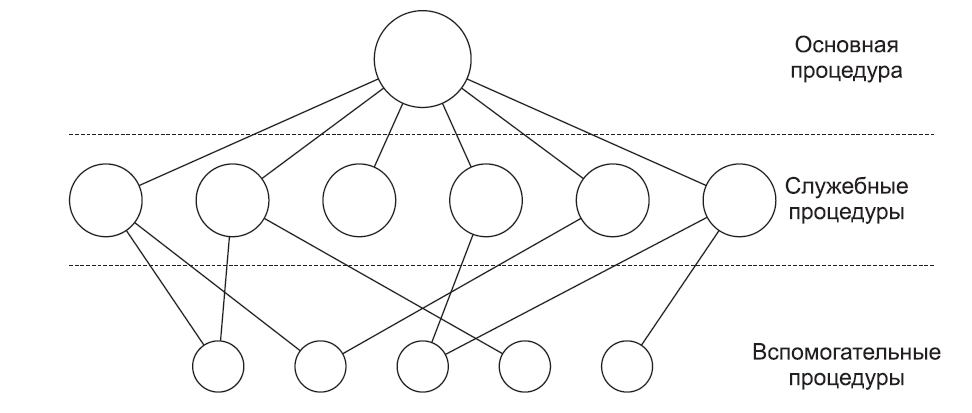
\includegraphics[scale=0.7]{pic2-3.png}
   \caption{Простая структурированная модель монолитной системы}
\end{figure}

Примеры: Традиционные ядра UNIX, такие как BSD; Linux.
\newline

\textbf{Модульное ядро}

\textit{Модульное ядро} — современная, усовершенствованная модификация архитектуры монолитных ядер операционных систем компьютеров.

В отличие от «классических» монолитных ядер, считающихся ныне устаревшими, модульные ядра, как правило, не требуют полной перекомпиляции ядра при изменении состава аппаратного обеспечения компьютера. Вместо этого модульные ядра предоставляют тот или иной механизм подгрузки модулей ядра, поддерживающих то или иное аппаратное обеспечение (например, драйверов). При этом подгрузка модулей может быть как динамической (выполняемой «на лету», без перезагрузки ОС, в работающей системе), так и статической (выполняемой при перезагрузке ОС после переконфигурирования системы на загрузку тех или иных модулей).

Все модули ядра работают в адресном пространстве ядра и могут пользоваться всеми функциями, предоставляемыми ядром. Поэтому модульные ядра продолжают оставаться монолитными.

Модульные ядра удобнее для разработки, чем традиционные монолитные ядра, не поддерживающие динамическую загрузку модулей, так как от разработчика не требуется многократная полная перекомпиляция ядра при работе над какой-либо его подсистемой или драйвером. Выявление, локализация, отладка и устранение ошибок при тестировании также облегчаются.

Модульные ядра предоставляют особый программный интерфейс (API) для связывания модулей с ядром, для обеспечения динамической подгрузки и выгрузки модулей. В свою очередь, не любая программа может быть сделана модулем ядра: на модули ядра накладываются определённые ограничения в части используемых функций (например, они не могут пользоваться функциями стандартной библиотеки С/С++ и должны использовать специальные аналоги, являющиеся функциями API ядра). Кроме того, модули ядра обязаны экспортировать определённые функции, нужные ядру для правильного подключения и распознавания модуля, для его корректной инициализации при загрузке и корректного завершения при выгрузке, для регистрации модуля в таблице модулей ядра и для обращения из ядра к сервисам, предоставляемым модулем.

Не все части ядра могут быть сделаны модулями. Некоторые части ядра всегда обязаны присутствовать в оперативной памяти и должны быть жёстко "вшиты" в ядро. Также не все модули допускают динамическую подгрузку (без перезагрузки ОС). Степень модульности ядер (количество и разнообразие кода, которое может быть вынесено в отдельные модули ядра и допускает динамическую подгрузку) различна в различных архитектурах модульных ядер. Ядра Linux в настоящее время имеют более модульную архитектуру, чем ядра *BSD (FreeBSD, NetBSD, OpenBSD).

Общей тенденцией развития современных модульных архитектур является всё большая модуларизация кода (повышение степени модульности ядер), улучшение механизмов динамической подгрузки и выгрузки, уменьшение или устранение необходимости в ручной подгрузке модулей или в переконфигурации ядра при изменениях аппаратуры путём введения тех или иных механизмов автоматического определения оборудования и автоматической подгрузки нужных модулей, универсализация кода ядра и введение в ядро абстрактных механизмов, предназначенных для совместного использования многими модулями (примером может служить VFS — «виртуальная файловая система», совместно используемая многими модулями файловых систем в ядре Linux).
\newline

\textbf{Микроядро}

\textit{Микроядро} — это минимальная реализация основных функций ядра операционной системы компьютера.

Классические микроядра предоставляют лишь очень небольшой набор низкоуровневых примитивов, или системных вызовов, реализующих наиболее базовые сервисы операционной системы. Сюда относятся управление адресным пространством оперативной и виртуальной памяти, управление процессами и тредами, а также средства межпроцессной коммуникации.
Все остальные сервисы ОС, в классических монолитных ядрах ОС предоставляемые непосредственно ядром, в микроядерных архитектурах реализуются в адресном пространстве пользователя и называются серверами. Примерами таких серверов, выносимых в пространство пользователя в микроядерных архитектурах, являются сетевые сервисы, файловая система.

Замысел, положенный в основу конструкции микроядра, направлен на достижение высокой надежности за счет разбиения операционной системы на небольшие, вполне определенные модули. Только один из них — микроядро — запускается в режиме ядра, а все остальные запускаются в виде относительно слабо наделенных полномочиями обычных пользовательских процессов. В частности, если запустить каждый драйвер устройства и файловую систему как отдельные пользовательские процессы, то ошибка в одном из них может вызвать отказ соответствующего компонента, но не сможет вызвать сбой всей системы. Таким образом, ошибка в драйвере звукового устройства приведет к искажению или пропаданию звука, но не вызовет зависания компьютера. В отличие от этого в монолитной системе, где все драйверы находятся в ядре, некорректный драйвер звукового устройства может запросто сослаться на неверный адрес памяти и привести систему к немедленной вынужденной остановке.

Такая конструкция позволяет сделать структуру ядра «истинно динамичной» и улучшить общее быстродействие системы (небольшое микроядро может уместится в монокристаллическом кэше процессора). Недостатком подобного подхода является плата за принудительное «переключение» процессов в ядре; этот факт собственно и объясняет трудности в проектировании и написании ядер подобной конструкции. Примеры операционных систем на основе микроядра: QNX, GNU Hurd, Minix3.

За пределами ядра структура системы представляет собой три уровня процессов, которые работают в режиме пользователя. Самый нижний уровень содержит драйверы устройств. Поскольку они работают в пользовательском режиме, у них нет физического доступа к пространству портов ввода-вывода и они не могут вызывать команды ввода-вывода напрямую. Вместо этого, чтобы запрограммировать устройство ввода-вывода, драйвер создает структуру, сообщающую, какие значения в какие порты ввода-вывода следует записать. Затем драйвер осуществляет вызов ядра, сообщая ядру, что нужно произвести запись. При этом ядро может осуществить проверку, использует ли драйвер то устройство ввода-вывода, с которым он имеет право работать. Следовательно (в отличие от монолитной конструкции), дефектный драйвер звукового устройства не может случайно осуществить запись на диск.

Над драйверами расположен уровень, содержащий службы, которые осуществляют основной объем работы операционной системы. Все они работают в режиме пользователя. Одна или более файловых служб управляют файловой системой (или системами), диспетчер процессов создает и уничтожает процессы, управляет ими и т. д. Пользовательские программы получают доступ к услугам операционной системы путем отправки коротких сообщений этим службам, которые запрашивают системные вызовы POSIX. Например, процесс, нуждающийся в выполнении вызова read, отправляет сообщение одной из файловых служб, предписывая ей, что нужно прочитать.

\begin{figure}\center
   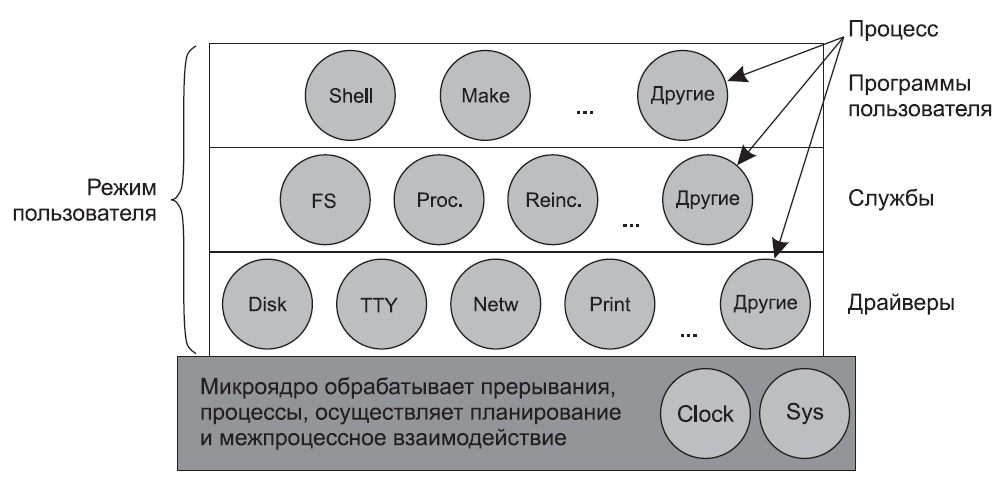
\includegraphics[scale=0.7]{pic2-4.png}
   \caption{Упрощенная структура системы MINIX 3}
\end{figure}

Особый интерес представляет служба перевоплощения (reincarnation server), выполняющая проверку функционирования других служб и драйверов. В случае обнаружения отказа одного из компонентов он автоматически заменяется без какого-либо вмешательства со стороны пользователя. Таким образом, система самостоятельно исправляет отказы и может достичь высокой надежности.
\newline

\textbf{Экзоядро}

\textit{Экзоядро} — ядро операционной системы компьютеров, предоставляющее лишь функции для взаимодействия между процессами и безопасного выделения и освобождения ресурсов.

\textit{Экзо — приставка, обозначающая нечто внешнее, находящееся снаружи.}

В традиционных операционных системах ядро предоставляет не только минимальный набор сервисов, обеспечивающих выполнение программ, но и большое количество высокоуровневых абстракций для использования разнородных ресурсов компьютера: оперативной памяти, жестких дисков, сетевых подключений. В отличие от них, ОС на основе экзоядра предоставляет лишь набор сервисов для взаимодействия между приложениями, а также необходимый минимум функций, связанных с защитой: выделение и высвобождение ресурсов, контроль прав доступа, и т. д. Экзоядро не занимается предоставлением абстракций для физических ресурсов — эти функции выносятся в библиотеку пользовательского уровня (так называемую libOS).

Основная идея операционной системы на основе экзоядра состоит в том, что ядро должно выполнять лишь функции координатора для небольших процессов, связанных только одним ограничением — экзоядро должно иметь возможность гарантировать безопасное выделение и освобождение ресурсов оборудования. В отличие от ОС на основе микроядра, ОС, базирующиеся на экзоядре, обеспечивают гораздо большую эффективность за счет отсутствия необходимости в переключении между процессами при каждом обращении к оборудованию.

Архитектуры на основе экзоядер являются дальнейшим развитием и усовершенствованием микроядерных архитектур и одновременно ужесточают требования к минималистичности и простоте кода ядра.

libOS может обеспечивать произвольный набор абстракций, совместимый с той или другой уже существующей операционной системой, например Linux или Windows.
\newline

\textbf{Клиент-серверная модель}

Небольшая вариация идеи микроядер выражается в обособлении двух классов процессов: серверов, каждый из которых предоставляет какую-нибудь службу, и клиентов, которые пользуются этими службами. Эта модель известна как клиент-серверная. Довольно часто самый нижний уровень представлен микроядром, но это не обязательно. Суть заключается в наличии клиентских процессов и серверных процессов.

Связь между клиентами и серверами часто организуется с помощью передачи сообщений. Чтобы воспользоваться службой, клиентский процесс составляет сообщение, в котором говорится, что именно ему нужно, и отправляет его соответствующей службе. Затем служба выполняет определенную работу и отправляет обратно ответ. Если клиент и сервер запущены на одной и той же машине, то можно провести определенную оптимизацию, но концептуально здесь речь идет о передаче сообщений.

Очевидным развитием этой идеи будет запуск клиентов и серверов на разных компьютерах соединенных локальной или глобальной сетью. Поскольку клиенты связываются с серверами путем отправки сообщений, им не обязательно знать, будут ли эти сообщения обработаны локально, на их собственных машинах, или же они будут отправлены по сети на серверы, расположенные на удаленных машинах. Что касается интересов клиента, следует отметить, что в обоих случаях происходит
одно и то же: отправляются запросы и возвращаются ответы. Таким образом, клиент-серверная модель является абстракцией, которая может быть использована как для отдельно взятой машины, так и для машин, объединенных в сеть.

\begin{figure}\center
   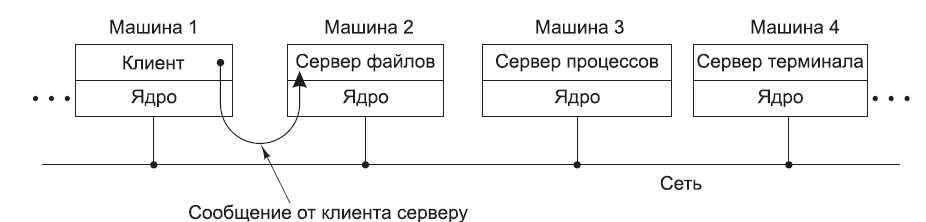
\includegraphics[scale=0.7]{pic2-5.png}
   \caption{Клиент-серверная модель, реализованная с помощью сети}
\end{figure}

\newpage
%------------------------------------------------------------------------------------
\chapter{Управление процессами в многозадачных ОС}
%-------------------------------------------------------------------------------------
%------------------------------ПРОЦЕССЫ И ПОТОКИ--------------------------------------
%-------------------------------------------------------------------------------------

\section{Процессы и потоки}
\subsection{Понятие процесса}

В первой лекции, поясняя понятие "операционная система" и описывая способы построения операционных систем, мы часто применяли слова "программа" и "задание". Мы говорили: вычислительная система исполняет одну или несколько программ, операционная система планирует задания, программы могут обмениваться данными и т. д. Мы использовали эти термины в некотором общеупотребительном, житейском смысле, предполагая, что все читатели одинаково представляют себе, что подразумевается под ними в каждом конкретном случае. При этом одни и те же слова обозначали и объекты в статическом состоянии, не обрабатывающиеся вычислительной системой (например, совокупность файлов на диске), и объекты в динамическом состоянии, находящиеся в процессе исполнения. Это было возможно, пока мы говорили об общих свойствах операционных систем, не вдаваясь в подробности их внутреннего устройства и поведения, или о работе вычислительных систем первого-второго поколений, которые не могли обрабатывать более одной программы или одного задания одновременно, по сути дела не имея операционных систем. Но теперь мы начинаем знакомиться с деталями функционирования современных компьютерных систем, и нам придется уточнить терминологию.

Рассмотрим следующий пример. Два студента запускают программу извлечения квадратного корня. Один хочет вычислить квадратный корень из 4, а второй – из 1. С точки зрения студентов, запущена одна и та же программа; с точки зрения компьютерной системы, ей приходится заниматься двумя различными вычислительными процессами, так как разные исходные данные приводят к разному набору вычислений. Следовательно, на уровне происходящего внутри вычислительной системы мы не можем использовать термин "программа" в пользовательском смысле слова.

Рассматривая системы пакетной обработки, мы ввели понятие "задание" как совокупность программы, набора команд языка управления заданиями, необходимых для ее выполнения, и входных данных. С точки зрения студентов, они, подставив разные исходные данные, сформировали два различных задания. Может быть, термин "задание" подойдет нам для описания внутреннего функционирования компьютерных систем? Чтобы выяснить это, давайте рассмотрим другой пример. Пусть оба студента пытаются извлечь корень квадратный из 1, то есть пусть они сформировали идентичные задания, но загрузили их в вычислительную систему со сдвигом по времени. В то время как одно из выполняемых заданий приступило к печати полученного значения и ждет окончания операции ввода-вывода, второе только начинает исполняться. Можно ли говорить об идентичности заданий внутри вычислительной системы в данный момент? Нет, так как состояние процесса их выполнения различно. Следовательно, и слово "задание" в пользовательском смысле не может применяться для описания происходящего в вычислительной системе.

Это происходит потому, что \textit{термины "программа" и "задание" предназначены для описания статических, неактивных объектов}. Программа же в процессе исполнения является динамическим, активным объектом. По ходу ее работы компьютер обрабатывает различные команды и преобразует значения переменных. Для выполнения программы операционная система должна выделить определенное количество оперативной памяти, закрепить за ней определенные устройства ввода-вывода или файлы (откуда должны поступать входные данные и куда нужно доставить полученные результаты), то есть зарезервировать определенные ресурсы из общего числа ресурсов всей вычислительной системы. Их количество и конфигурация с течением времени могут изменяться. Для описания таких активных объектов внутри компьютерной системы вместо терминов "программа" и "задание" мы будем использовать новый термин – "процесс".

\begin{opr}
   Процесс (или по-другому, задача) - абстракция, описывающая выполняющуюся программу. Для операционной системы процесс представляет собой единицу работы, заявку на потребление системных ресурсов. Подсистема управления процессами планирует выполнение процессов, то есть распределяет процессорное время между несколькими одновременно существующими в системе процессами, а также занимается созданием и уничтожением процессов, обеспечивает процессы необходимыми системными ресурсами, поддерживает взаимодействие между процессами.
\end{opr}

\textit{Понятие процесса} характеризует некоторую совокупность набора исполняющихся команд, ассоциированных с ним ресурсов (выделенная для исполнения память или адресное пространство, стеки, используемые файлы и устройства ввода-вывода и т. д.) и текущего момента его выполнения (значения регистров, программного счетчика, состояние стека и значения переменных), находящуюся под управлением операционной системы.

Не существует взаимно-однозначного соответствия между процессами и программами, обрабатываемыми вычислительными системами. Как будет показано далее, в некоторых операционных системах для работы определенных программ может организовываться более одного процесса или один и тот же процесс может исполнять последовательно несколько различных программ. Более того, даже в случае обработки только одной программы в рамках одного процесса нельзя считать, что процесс представляет собой просто динамическое описание кода исполняемого файла, данных и выделенных для них ресурсов. Процесс находится под управлением операционной системы, поэтому в нем может выполняться часть кода ее ядра (не находящегося в исполняемом файле!), как в случаях, специально запланированных авторами программы (например, при использовании системных вызовов), так и в непредусмотренных ситуациях (например, при обработке внешних прерываний).

%-------------------------------------------------------------------------------------
\subsection{Контекст и дескриптор процесса}
В основе UNIX лежит концепция процесса - единицы управления и единицы потребления ресурсов. Процесс представляет собой программу в состоянии выполнения, причем в UNIX в рамках одного процесса не могут выполняться никакие параллельные действия.

Каждый процесс работает в своем виртуальном адресном пространстве. Совокупность участков физической памяти, отображаемых на виртуальные адреса процесса, называется образом процесса.

При управлении процессами операционная система использует два основных типа информационных структур: дескриптор процесса (структура proc) и контекст процесса (структура user).

\textbf{\textit{Дескриптор процесса}} содержит такую информацию о процессе, которая необходима ядру в течение всего жизненного цикла процесса, независимо от того, находится ли он в активном или пассивном состоянии, находится ли образ процесса в оперативной памяти или выгружен на диск. Дескрипторы отдельных процессов объединены в список, образующий таблицу процессов. Память для таблицы процессов отводится динамически в области ядра. На основании информации, содержащейся в таблице процессов, операционная система осуществляет планирование и синхронизацию процессов. В дескрипторе прямо или косвенно (через указатели на связанные с ним структуры) содержится информация о состоянии процесса, расположении образа процесса в оперативной памяти и на диске, о значении отдельных составляющих приоритета, а также его итоговое значение - глобальный приоритет, идентификатор пользователя, создавшего процесс, информация о родственных процессах, о событиях, осуществления которых ожидает данный процесс и некоторая другая информация.

\textbf{\textit{Контекст процесса }} содержит менее оперативную, но более объемную часть информации о процессе, необходимую для возобновления выполнения процесса с прерванного места: содержимое регистров процессора, коды ошибок выполняемых процессором системных вызовов, информацию о всех открытых данным процессом файлов и незавершенных операциях ввода-вывода (указатели на структуры file) и другие данные, характеризующие состояние вычислительной среды в момент прерывания. Контекст, так же как и дескриптор процесса, доступен только программам ядра, то есть находится в виртуальном адресном пространстве операционной системы, однако он хранится не в области ядра, а непосредственно примыкает к образу процесса и перемещается вместе с ним, если это необходимо, из оперативной памяти на диск. В UNIX для процессов предусмотрены два режима выполнения: привилегированный режим - "система" и обычный режим - "пользователь". В режиме "пользователь" запрещено выполнение действий, связанных с управлением ресурсами системы, в частности, корректировка системных таблиц, управление внешними устройствами, маскирование прерываний, обработка прерываний. В режиме "система" выполняются программы ядра, а в режиме "пользователь" - оболочка и прикладные программы. При необходимости выполнить привилегированные действия пользовательский процесс обращается с запросом к ядру в форме так называемого системного вызова. В результате системного вызова управление передается соответствующей программе ядра. С момента начала выполнения системного вызова процесс считается системным. Таким образом, один и тот же процесс может находиться в пользовательской и системной фазах. Эти фазы никогда не выполняются одновременно.

В данных версиях UNIX процесс, работающий в режиме системы, не мог быть вытеснен другим процессом. Из-за этого организация ядра, которое составляет привилегированную общую часть всех процессов, упрощалась, т.к. все функции ядра не были реентерабельными. Однако, при этом реактивность системы страдала - любой процесс, даже низкоприоритетный, войдя в системную фазу, мог оставаться в ней сколь угодно долго. Из-за этого свойства UNIX не мог использоваться в качестве ОС реального времени. В более поздних версиях, и в SVR4 в том числе, организация ядра усложнилась и процесс можно вытеснить и в системной фазе, но не в произвольный момент времени, а только в определенные периоды его работы, когда процесс сам разрешает это сделать установкой специального сигнала.

В SVR4 имеется несколько процессов, которые не имеют пользовательской фазы, например, процесс pageout, организующий выталкивание страниц на диск.

Порождение процессов в системе UNIX происходит следующим образом. При создании процесса строится образ порожденного процесса, являющийся точной копией образа породившего процесса. Сегмент данных и сегмент стека отца действительно копируются на новое место, образуя сегменты данных и стека сына. Процедурный сегмент копируется только тогда, когда он не является разделяемым. В противном случае сын становится еще одним процессом, разделяющим данный процедурный сегмент.

После выполнения системного вызова fork оба процесса продолжают выполнение с одной и той же точки. Чтобы процесс мог опознать, является ли он отцом или сыном, системный вызов fork возвращает в качестве своего значения в породивший процесс идентификатор порожденного процесса, а в порожденный процесс NULL. Типичное разветвление на языке C записывается так:
\begin{lstlisting}
      if ( fork() ) //parent action
      else   //child action  
\end{lstlisting}

Идентификатор сына может быть присвоен переменной, входящей в контекст процесса-отца. Так как контекст процесса наследуется его потомками, то дети могут узнать идентификаторы своих старших братьев, так образом сумма знаний наследуется при порождении и может быть распространена между родственными процессами. Наследуются все характеристики процесса, содержащиеся в контексте.

На независимости идентификатора процесса от выполняемой процессом программы построен механизм, позволяющий процессу придти к выполнению другой программы с помощью системного вызова exec.

Таким образом в UNIX порождение нового процесса происходит в два этапа - сначала создается копия процесса-родителя, то есть дублируется дескриптор, контекст и образ процесса. Затем у нового процесса производится замена кодового сегмента на заданный.

Вновь созданному процессу операционная система присваивает целочисленный идентификатор, уникальный за весь период функционирования системы.
%-------------------------------------------------------------------------------------
\subsection{Классификация процессов}

\begin{figure}\center
   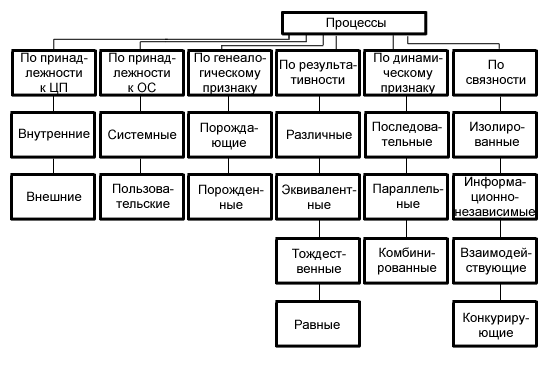
\includegraphics[scale=1.3]{pic3-1.png}
\end{figure}

\textbf{По временным признакам}

Процессы определяются рядом временных характеристик. В некоторый момент времени процесс может быть порожден (образован), а через некоторое время закончен. Интервал между этими моментами называют интервалом существования процесса.

В момент порождения последовательность и длительность пребывания процесса в каждом из своих состояний (трасса процесса) в общем случае непредсказуемы. Следовательно, непредсказуема и длительность интервала существования. Однако отдельные виды процессов требуют такого планирования, чтобы гарантировать окончание процесса до наступления некоторого конкретного момента времени. Процессы такого класса называют процессами реального времени. В другой класс входят процессы, время существования которых должно быть не более интервала времени допустимой реакции ЭВМ на запросы пользователя. Процессы такого класса называют интерактивными. Процессы, не вошедшие в эти классы, называют пакетными.
\newline

\textbf{По генеалогическому признаку}

В любой ОС по требованию существующего или существовавшего процесса проводится работа по порождению процессов. Процесс, задающий данное требование, называют порождающим, а создаваемый по требованию — порожденным. Если порожденный процесс на интервале своего существования в свою очередь выдает требование на порождение другого процесса, то он одновременно становится и порождающим.

При управлении процессами важно обеспечить воспроизводимость результатов работы каждого процесса, учитывать и управлять той ситуацией, которая складывалась при развитии процесса. Поэтому часто для оказывается важен не только результат счета, но и каким образом этот результат достигается. С этих позиций ОС сравнивает процессы по динамическим свойствам, используя понятие "трасса"—порядок и длительность пребывания процесса в допустимых состояниях на интервале существования.
\newline

\textbf{По результативности}

Два процесса, которые имеют одинаковый конечный результат обработки одних и тех же исходных данных по одной и той же или даже различным программам на одном и том же или на различных процессорах, называют эквивалентными. Трассы эквивалентных процессов в общем случае не совпадают. Если в каждом из эквивалентных процессов обработка данных происходит по одной и той же программе, но трассы при этом в общем случае не совпадают, то такие процессы называют тождественными. При совпадении трасс у тождественных процессов их называют равными. Во всех остальных случаях процессы всегда различны.
\newline

\textbf{По динамическим признакам}

Проблематичность управления процессами заключается в том, что в момент порождения процессов их трассы неизвестны. Кроме того, требуется учитывать, каким образом соотносятся во времени интервалы существования процессов. Если интервалы двух процессов не пересекаются во времени, то такие два процесса называют последовательными друг относительно друга. Если на рассматриваемом интервале времени существуют одновременно два процесса, то они на этом интервале являются параллельными друг относительно друга. Если на рассматриваемом интервале найдется хотя бы одна точка, в которой существует один процесс, но не существует другой, и хотя бы одна точка, в которой оба процесса существуют одновременно, то такие два процесса называют комбинированными.
\newline

\textbf{По принадлежности к ЦП}

В операционной системе принято различать процессы не только по времени, но и по месту их развития, т. е. на каком из процессоров исполняется программа процесса. Точкой отсчета принято считать центральный процессор (процессоры), на котором развиваются процессы, называемые программными или внутренними. Такое название указывает на возможность существования в системе процессов, называемых внешними. Это процессы, развитие которых происходит под контролем или управлением ОС на процессорах, отличных от центрального. Ими могут быть, например, процессы ввода — вывода, развивающиеся в канале. Деятельность любого пользователя ЭВМ, который в том или ином виде вводит посредством ОС информацию, требуемую для исполнения одной или нескольких программ, можно также рассматривать как внешний процесс.
\newline

\textbf{По принадлежности к ОС}

Программные процессы принято делить на системные и пользовательские. При развитии системного процесса исполняется программа из состава операционной системы. При развитии пользовательского процесса исполняется пользовательская (прикладная) программа.
\newline

\textbf{По связности}

Процессы независимо от их вида могут быть взаимосвязанными или изолированными друг от друга. Два процесса являются взаимосвязанными, если между ними поддерживаются с помощью системы управления процессами какого-либо рода связи: функциональные, пространственно-временные, управляющие, информационные и т. д. В противном случае они являются изолированными (точнее - процессами со слабыми связями, так как при отсутствии явных связей они могут быть связаны косвенно и определенным образом влиять на развитие друг друга).

При наличии между процессами управляющей связи устанавливается отношение вида "порождающий—порождаемый", рассмотренное выше. Если два взаимосвязанных процесса при развитии используют совместно некоторые ресурсы, но информационно между собой не связаны, т. е. не обмениваются информацией, то такие процессы называют информационно-независимыми. Связь между такими процессами может быть либо функциональная, либо пространственно-временная. При наличии информационных связей между двумя процессами их называют взаимодействующими, причем схемы, а следовательно, и механизмы установления таких связей могут быть различными. Особенность, во-первых, обусловлена динамикой процессов (т. е. являются ли взаимодействующие процессы последовательными, параллельными или комбинированными); во-вторых, выбранным способом связи (явным, с помощью явного обмена сообщениями между процессами, или неявным, с помощью разделяемых структур данных). Когда необходимо подчеркнуть связь между взаимосвязанными процессами по ресурсам, их называют конкурирующими.

%-------------------------------------------------------------------------------------
\subsection{Диаграмма состояния процесса}

В многозадачной (многопроцессной) системе процесс может находиться в одном из трех основных состояний:

\begin{opr}
   ВЫПОЛНЕНИЕ - активное состояние процесса, во время которого процесс обладает всеми необходимыми ресурсами и непосредственно выполняется процессором;
\end{opr}

\begin{opr}
   ОЖИДАНИЕ - пассивное состояние процесса, процесс заблокирован, он не может выполняться по своим внутренним причинам, он ждет осуществления некоторого события, например, завершения операции ввода-вывода, получения сообщения от другого процесса, освобождения какого-либо необходимого ему ресурса;
\end{opr}

\begin{opr}
   ГОТОВНОСТЬ - также пассивное состояние процесса, но в этом случае процесс заблокирован в связи с внешними по отношению к нему обстоятельствами: процесс имеет все требуемые для него ресурсы, он готов выполняться, однако процессор занят выполнением другого процесса.
\end{opr}

В ходе жизненного цикла каждый процесс переходит из одного состояния в другое в соответствии с алгоритмом планирования процессов, реализуемым в данной операционной системе. Типичный граф состояний процесса показан на рисунке:

\begin{figure}[!h]\center
   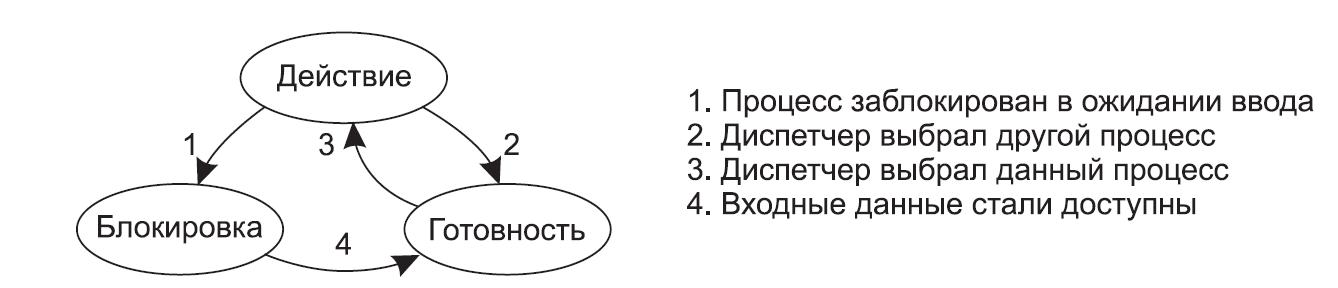
\includegraphics[scale=0.55]{pic3-2.png}
\end{figure}

В состоянии ВЫПОЛНЕНИЕ в однопроцессорной системе может находиться только один процесс, а в каждом из состояний ОЖИДАНИЕ и ГОТОВНОСТЬ - несколько процессов, эти процессы образуют очереди соответственно ожидающих и готовых процессов. Жизненный цикл процесса начинается с состояния ГОТОВНОСТЬ, когда процесс готов к выполнению и ждет своей очереди. При активизации процесс переходит в состояние ВЫПОЛНЕНИЕ и находится в нем до тех пор, пока либо он сам освободит процессор, перейдя в состояние ОЖИДАНИЯ какого-нибудь события, либо будет насильно "вытеснен" из процессора, например, вследствие исчерпания отведенного данному процессу кванта процессорного времени. В последнем случае процесс возвращается в состояние ГОТОВНОСТЬ. В это же состояние процесс переходит из состояния ОЖИДАНИЕ, после того, как ожидаемое событие произойдет.
\newpage
%-------------------------------------------------------------------------------------
\subsection{Многопоточность. Понятие потока}

\begin{opr}
   Многопоточность — свойство операционной системы, заключающееся в том, что задача может выполняться в более чем 1 потоке, за счёт чего достигается более эффективное использование ресурсов вычислительной машины. Как правило, операционные системы, реализующие многозадачность, реализуют и многопоточность.
\end{opr}


Сутью многопоточности является квазимногозадачность на уровне одного исполняемого процесса, то есть все потоки выполняются в адресном пространстве процесса. На момент выполнения процесса он имеет как минимум один (главный) поток.

К достоинствам многопоточности в программировании можно отнести следующее:
\begin{itemize}
   \item Упрощение программы в некоторых случаях, за счет использования общего адресного пространства.
   \item Быстрота создания потока, по сравнению с процессом, примерно в 100 раз.
   \item Повышение производительности самой программы, т.к. есть возможность одновременно выполнять вычисления на процессоре и операцию ввода/вывода. Пример: текстовый редактор с тремя потоками может одновременно взаимодействовать с пользователем, форматировать текст и записывать на диск резервную копию.
\end{itemize}

Каждому процессу соответствует адресное пространство и одиночный поток исполняемых команд. В многопользовательских системах, при каждом обращении к одному и тому же сервису, приходится создавать новый процесс для обслуживания клиента. Это менее выгодно, чем создать квазипараллельный поток внутри этого процесса с одним адресным пространством.



Каждому процессу соответствует адресное пространство и одиночный поток исполняемых команд. В многопользовательских системах, при каждом обращении к одному и тому же сервису, приходится создавать новый процесс для обслуживания клиента. Это менее выгодно, чем создать квазипараллельный поток внутри этого процесса с одним адресным пространством.
\begin{figure}[!h]\center
   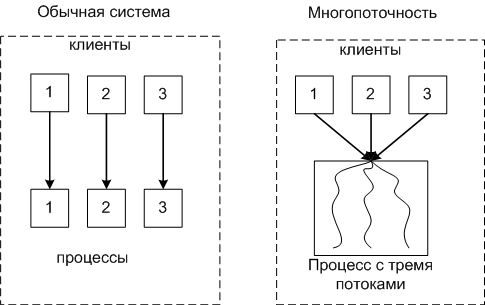
\includegraphics[scale=1.1]{pic3-3.png}
   \caption{Сравнение многопоточной системы с однопоточной}
\end{figure}

С каждым потоком связывается:
\begin{itemize}
   \item Счетчик выполнения команд
   \item Регистры для текущих переменных
   \item Стек
   \item Состояние
   \item Потоки делят между собой элементы своего процесса:
   \item Адресное пространство
   \item Глобальные переменные
   \item Открытые файлы
   \item Таймеры
   \item Семафоры
   \item Статистическую информацию.
\end{itemize}
\begin{figure}[!h]\center
   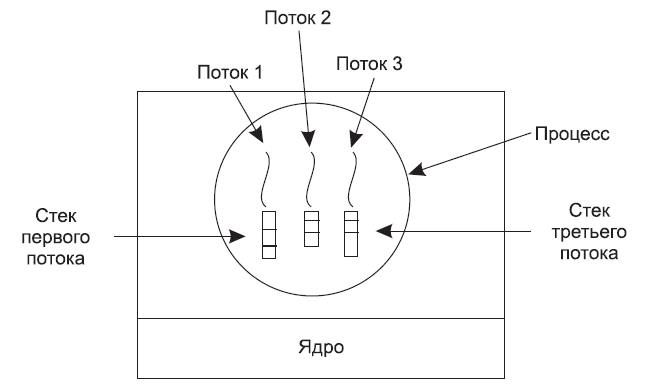
\includegraphics[scale=1]{pic3-5.png}
   \caption{У каждого потока имеется собственный стек}
\end{figure}
В остальном модель иеднтична модели процессов.
В Windows есть поддержка потоков на уровне ядра. В Linux есть новый системный вызов clone для создания потоков, отсутствующий во всех остальных версиях системы UNIX.
\newpage
%-------------------------------------------------------------------------------------
\subsection{Способы реализации потока}
\begin{figure}[!h]\center
   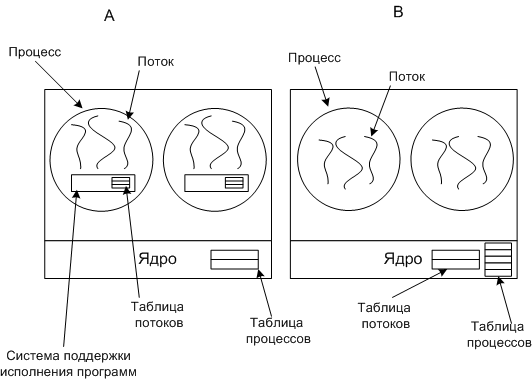
\includegraphics[scale=1]{pic3-4.png}
   \caption{А - потоки в пространстве пользователя
      B - потоки в пространстве ядра}
\end{figure}
\textbf{Поток в пространстве пользователя}

Каждый процесс имеет таблицу потоков, аналогичную таблице процессов ядра. В этом случае ядро о потоках ничего не знает.

\textit{\textbf{Преимущества:}}

\begin{itemize}
   \item Такую многопоточность можно реализовать на ядре не поддерживающим многопоточность
   \item Более быстрое переключение, создание и завершение потоков
   \item Процесс может иметь собственный алгоритм планирования.
\end{itemize}

\textit{\textbf{Недостатки:}}
\begin{itemize}
   \item Отсутствие прерывания по таймеру внутри одного процесса
   \item При использовании блокирующего (процесс переводится в режим ожидания, например: чтение с клавиатуры, а данные не поступают) системного запроса все остальные потоки блокируются.
   \item Сложность реализации
\end{itemize}

\textbf{Поток в пространстве ядра}

Все вызовы, способные заблокировать поток, реализованы как системные, с более существенными затратами, чем вызов процедуры в системе поддержки исполнения программ. Когда поток блокируется, ядро по своему выбору может запустить либо другой поток из этого же самого процесса (если имеется готовый к выполнению поток), либо поток из другого процесса. Когда потоки реализуются на пользовательском уровне, система поддержки исполнения программ работает с запущенными потоками собственного процесса до тех пор, пока ядро не заберет у нее центральный процессор (или не останется ни одного готового к выполнению потока).

Поскольку создание и уничтожение потоков в ядре требует относительно более весомых затрат, некоторые системы с учетом складывающейся ситуации применяют более правильный подход и используют свои потоки повторно. При уничтожении потока он помечается как неспособный к выполнению, но это не влияет на его структуру данных, имеющуюся в ядре. Чуть позже, когда должен быть создан новый поток, вместо этого повторно активируется старый поток, что приводит к экономии времени. Повторное использование потоков допустимо и на пользовательском уровне, но для этого нет достаточно веских оснований, поскольку издержки на управление потоками там значительно меньше.

Для потоков, реализованных на уровне ядра, не требуется никаких новых, неблокирующих системных вызовов. Более того, если один из выполняемых потоков столкнется с ошибкой обращения к отсутствующей странице, ядро может с легкостью проверить наличие у процесса любых других готовых к выполнению потоков и при наличии таковых запустить один из них на выполнение, пока будет длиться ожидание извлечения запрошенной страницы с диска. Главный недостаток этих потоков состоит в весьма существенных затратах времени на системный вызов, поэтому, если операции над потоками (создание, удаление и т. п.) выполняются довольно часто, это влечет за собой более существенные издержки.

Хотя потоки, создаваемые на уровне ядра, и позволяют решить ряд проблем, но справиться со всеми существующими проблемами они не в состоянии. Что будет, к примеру, когда произойдет разветвление многопоточного процесса? Будет ли у нового
процесса столько же потоков, сколько у старого, или только один поток? Во многих случаях наилучший выбор зависит от того, выполнение какого процесса запланировано следующим. Если он собирается вызвать команду exec, чтобы запустить новую программу, то, наверное, правильным выбором будет наличие только одного потока. Но если он продолжит выполнение, то лучше всего было бы, наверное, воспроизвести все имеющиеся потоки.

\textbf{Смешанная реализация}

В попытках объединить преимущества создания потоков на уровне пользователя и на
уровне ядра была исследована масса различных путей. Один из них заклю чается в использовании потоков на уровне ядра, а затем нескольких потоков на уровне пользователя в рамках некоторых или всех потоков на уровне ядра. При использовании такого подхода программист может определить, сколько потоков использовать на уровне ядра и на сколько потоков разделить каждый из них на уровне пользователя. Эта модель обладает максимальной гибкостью.

При таком подходе ядру известно только о потоках самого ядра, работу которых оно
и планирует. У некоторых из этих потоков могут быть несколько потоков на пользовательском уровне, которые расходятся от их вершины. Создание, удаление и планирование выполнения этих потоков осуществляется точно так же, как и у пользовательских
потоков, принадлежащих процессу, запущенному под управлением операционной
системы, не способной на многопоточную работу. В этой модели каждый поток на
уровне ядра обладает определенным набором потоков на уровне пользователя, которые
используют его по очереди.

\begin{figure}[!h]\center
   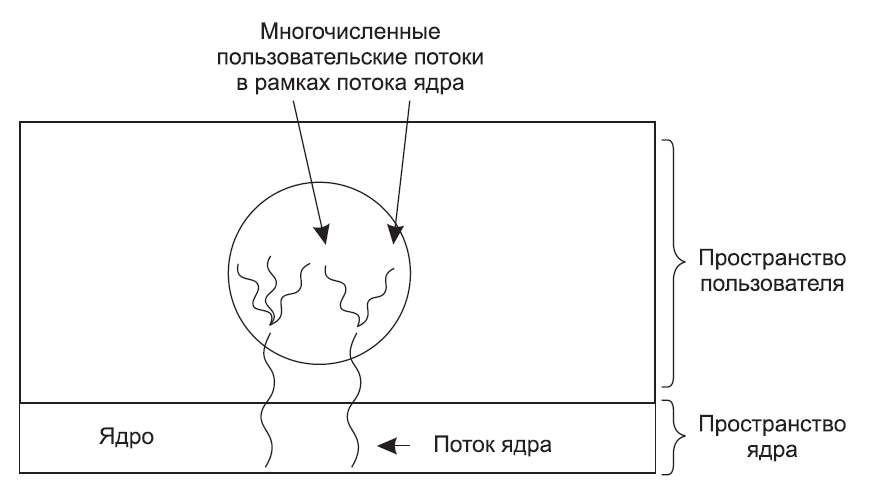
\includegraphics[scale=0.75]{pic3-6.png}
   \caption{Разделение на пользовательские потоки в рамках потока ядра}
\end{figure}

\textbf{Всплывающие потоки}

Потоки часто используются в распределенных системах. Хорошим примером может послужить обработка входящих сообщений, к примеру запросов на обслуживание. Традиционный подход заключается в использовании процесса или потока, блокирующегося системным вызовом receive в ожидании входящего сообщения. По прибытии сообщения он его принимает, распаковывает, проверяет его содержимое и проводит дальнейшую обработку.

Возможен и совершенно иной подход, при котором поступление сообщения вынуждает
систему создать новый поток для его обработки. Такой поток называется что они создаются заново и не имеют прошлого — никаких регистров, стека и всего остального, что должно быть восстановлено. Каждый такой поток начинается с чистого листа, и каждый их них идентичен всем остальным. Это позволяет создавать такие потоки довольно быстро. Новый поток получает сообщение для последующей обработки. В результате использования всплывающих потоков задержку между поступлением и началом обработки сообщения можно свести к минимуму.

\begin{figure}[!h]\center
   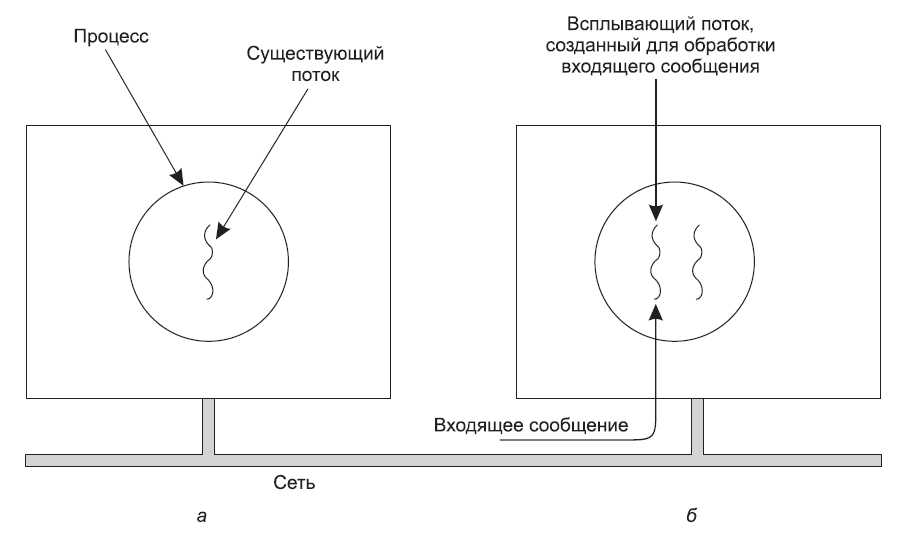
\includegraphics[scale=0.75]{pic3-7.png}
   \caption{Создание нового потока при поступлении сообщения:
      а — до поступления; б — после поступления}
\end{figure}

При использовании всплывающих потоков требуется предварительное планирование. К примеру, возникает вопрос: в каком процессе следует запускать поток? Если система поддерживает потоки, выполняемые в пространстве ядра, поток может быть запущен в этом пространстве. Как правило, запустить всплывающий поток в пространстве ядра легче и быстрее, чем поместить его в пользовательское пространство. К тому же всплывающий поток в пространстве ядра получает простой доступ ко всем таблицам ядра и к устройствам ввода-вывода, которые могут понадобиться для обработки прерывания. В то же время дефектный поток в пространстве ядра может нанести более существенный урон,
чем такой же поток в пространстве пользователя. К примеру, если он выполняется слишком долго, а способов его вытеснения не существует, входные данные могут быть утрачены навсегда.

\newpage
%-------------------------------------------------------------------------------------
%------------------------------ПЛАНИРОВАНИЕ ПРОЦЕССОВ---------------------------------
%-------------------------------------------------------------------------------------
\section{Планирование процессов}

\subsection{Планирование и диспетчеризация процессов}

Когда компьютер работает в многозадачном режиме, на нем зачастую запускается сра-
зу несколько процессов или потоков, претендующих на использование центрального
процессора. Такая ситуация складывается в том случае, если в состоянии готовности
одновременно находятся два или более процесса или потока. Если доступен только
один центральный процессор, необходимо выбрать, какой из этих процессов будет
выполняться следующим. Та часть операционной системы, на которую возложен этот
выбор, называется планировщиком, а алгоритм, который ею используется, называется
алгоритмом планирования.

В первой лекции, рассматривая эволюцию компьютерных систем, мы говорили о двух видах планирования в вычислительных системах: планировании заданий и планировании использования процессора. Планирование заданий появилось в пакетных системах после того, как для хранения сформированных пакетов заданий начали использоваться магнитные диски. Магнитные диски, являясь устройствами прямого доступа, позволяют загружать задания в компьютер в произвольном порядке, а не только в том, в котором они были записаны на диск. Изменяя порядок загрузки заданий в вычислительную систему, можно повысить эффективность ее использования. \textit{Процедуру выбора очередного задания для загрузки в машину, т. е. для порождения соответствующего процесса, мы и назвали планированием заданий.} Планирование использования процессора впервые возникает в мультипрограммных вычислительных системах, где в состоянии готовность могут одновременно находиться несколько процессов. Именно для процедуры выбора из них одного процесса, который получит процессор в свое распоряжение, т. е. будет переведен в состояние исполнение, мы использовали это словосочетание. Теперь, познакомившись с концепцией процессов в вычислительных системах, оба вида планирования мы будем рассматривать как различные уровни планирования процессов.

\textit{Планирование заданий используется в качестве долгосрочного планирования процессов. Оно отвечает за порождение новых процессов в системе, определяя ее степень мультипрограммирования, т. е. количество процессов, одновременно находящихся в ней.}Если степень мультипрограммирования системы поддерживается постоянной, т. е. среднее количество процессов в компьютере не меняется, то новые процессы могут появляться только после завершения ранее загруженных. Поэтому долгосрочное планирование осуществляется достаточно редко, между появлением новых процессов могут проходить минуты и даже десятки минут. Решение о выборе для запуска того или иного процесса оказывает влияние на функционирование вычислительной системы на протяжении достаточно длительного времени. Отсюда и название этого уровня планирования – долгосрочное. В некоторых операционных системах долгосрочное планирование сведено к минимуму или отсутствует вовсе. Так, например, во многих интерактивных системах разделения времени порождение процесса происходит сразу после появления соответствующего запроса. Поддержание разумной степени мультипрограммирования осуществляется за счет ограничения количества пользователей, которые могут работать в системе, и особенностей человеческой психологии. Если между нажатием на клавишу и появлением символа на экране проходит 20–30 секунд, то многие пользователи предпочтут прекратить работу и продолжить ее, когда система будет менее загружена.

\textit{Планирование использования процессора применяется в качестве краткосрочного планирования процессов.} Оно проводится, к примеру, при обращении исполняющегося процесса к устройствам ввода-вывода или просто по завершении определенного интервала времени. Поэтому краткосрочное планирование осуществляется, как правило, не реже одного раза в 100 миллисекунд. Выбор нового процесса для исполнения оказывает влияние на функционирование системы до наступления очередного аналогичного события, т. е. в течение короткого промежутка времени, чем и обусловлено название этого уровня планирования – краткосрочное.

В некоторых вычислительных системах бывает выгодно для повышения производительности временно удалить какой-либо частично выполнившийся процесс из оперативной памяти на диск, а позже вернуть его обратно для дальнейшего выполнения. Такая процедура в англоязычной литературе получила название \textit{swapping}, что можно перевести на русский язык как "перекачка", хотя в специальной литературе оно употребляется без перевода – свопинг. Когда и какой из процессов нужно перекачать на диск и вернуть обратно, решается дополнительным промежуточным уровнем планирования процессов – среднесрочным.
Процесс планирования осуществляется частью операционной системы, называемой планировщиком.

Диспетчеризация заключается в реализации найденного в результате планирования (динамического или статического) решения, т.е. в переключении процессора с одного потока на другой. Прежде чем прервать выполнение потока, ОС запоминает его контекст, с тем чтобы впоследствии использовать эту информацию для последующего возобновления выполнения данного потока. Контекст отражает, во-первых, состояние аппаратуры компьютера в момент прерывания потока: значение счетчика команд, содержимое регистров общего назначения, режим работы процессора, флаги, маски прерываний и другие параметры. Во-вторых, контекст включает параметры операционной среды, а именно ссылки на открытые файлы, данные о незавершенных операциях ввода- вывода, коды ошибок выполняемых данным потоком системных вызовов и т.д.

Диспетчеризация сводится к следующему:
\begin{itemize}
   \item сохранение контекста текущего потока, который требуется сменить;
   \item загрузка контекста нового потока, выбранного в результате планирования;
   \item запуск нового потока на выполнение.
\end{itemize}

Поскольку операция переключения контекстов существенно влияет на производительность вычислительной системы, программные модули ОС выполняют диспетчеризацию потоков совместно с аппаратными средствами процессора.
\newpage
%-------------------------------------------------------------------------------------
\subsection{Планирование и диспетчеризация процессов}

Вытесняющее и невытесняющее планирование
Планировщик может принимать решения о выборе для исполнения нового процесса из числа находящихся в состоянии готовность в следующих четырех случаях.

\begin{itemize}
   \item Когда процесс переводится из состояния исполнение в состояние закончил исполнение.
   \item Когда процесс переводится из состояния исполнение в состояние ожидание.
   \item Когда процесс переводится из состояния исполнение в состояние готовность (например, после прерывания от таймера).
   \item  Когда процесс переводится из состояния ожидание в состояние готовность (завершилась операция ввода-вывода или произошло другое событие).
\end{itemize}

В случаях 1 и 2 процесс, находившийся в состоянии исполнение, не может дальше исполняться, и операционная система вынуждена осуществлять планирование выбирая новый процесс для выполнения. В случаях 3 и 4 планирование может как проводиться, так и не проводиться, планировщик не вынужден обязательно принимать решение о выборе процесса для выполнения, процесс, находившийся в состоянии исполнение может просто продолжить свою работу. Если в операционной системе планирование осуществляется только в вынужденных ситуациях, говорят, что имеет место невытесняющее \textit{(nonpreemptive)} планирование. Если планировщик принимает и вынужденные, и невынужденные решения, говорят о вытесняющем \textit{(preemptive)} планировании. Термин "вытесняющее планирование" возник потому, что исполняющийся процесс помимо своей воли может быть вытеснен из состояния исполнение другим процессом.

\textbf{Невытесняющее планирование} используется, например, в MS Windows 3.1 и ОС Apple Macintosh. При таком режиме планирования процесс занимает столько процессорного времени, сколько ему необходимо. При этом переключение процессов возникает только при желании самого исполняющегося процесса передать управление (для ожидания завершения операции ввода-вывода или по окончании работы). Этот метод планирования относительно просто реализуем и достаточно эффективен, так как позволяет выделить большую часть процессорного времени для работы самих процессов и до минимума сократить затраты на переключение контекста. Однако при невытесняющем планировании возникает проблема возможности полного захвата процессора одним процессом, который вследствие каких-либо причин (например, из-за ошибки в программе) зацикливается и не может передать управление другому процессу. В такой ситуации спасает только перезагрузка всей вычислительной системы.

\textbf{Вытесняющее планирование} обычно используется в системах разделения времени. В этом режиме планирования процесс может быть приостановлен в любой момент исполнения. Операционная система устанавливает специальный таймер для генерации сигнала прерывания по истечении некоторого интервала времени – кванта. После прерывания процессор передается в распоряжение следующего процесса. Временные прерывания помогают гарантировать приемлемое время отклика процессов для пользователей, работающих в диалоговом режиме, и предотвращают "зависание" компьютерной системы из-за зацикливания какой-либо программы
\newpage
%-------------------------------------------------------------------------------------
\subsection{Планирование в системах пакетной обработки данных – дисциплины FCFS, SJN, SRT}

\textbf{FCFS}

Наверное, наипростейшим из всех алгоритмов планирования будет неприоритетный
алгоритм, следующий принципу «первым пришел — первым обслужен». При исполь-
зовании этого алгоритма центральный процессор выделяется процессам в порядке
поступления их запросов. По сути, используется одна очередь процессов, находящихся
в состоянии готовности. Когда рано утром в систему извне попадает первое задание,
оно тут же запускается на выполнение и получает возможность выполняться как угод-
но долго. Оно не прерывается по причине слишком продолжительного выполнения.
Другие задания по мере поступления помещаются в конец очереди. При блокировке
выполняемого процесса следующим запускается первый процесс, стоящий в очереди.
Когда заблокированный процесс переходит в состояние готовности, он, подобно толь-
ко что поступившему заданию, помещается в конец очереди, после всех ожидающих
процессов.

Сильной стороной этого алгоритма является простота его понимания и такая же
простота его программирования. Его справедливость сродни справедливости рас-
пределения дефицитных билетов на спортивные или концертные зрелища или мест
в очереди на новые айфоны тем людям, которые заняли очередь с двух часов ночи.
При использовании этого алгоритма отслеживание готовых процессов осуществляется
с помощью единого связанного списка. Выбор следующего выполняемого процесса
сводится к извлечению одного процесса из начала очереди. Добавление нового задания
или разблокированного процесса сводится к присоединению его к концу очереди. Что
может быть проще для восприятия и реализации?

К сожалению, принцип «первым пришел — первым обслужен» страдает и существен-
ными недостатками. Предположим, что используются один процесс, ограниченный
скоростью вычислений, который всякий раз запускается на 1 с, и множество процессов,
ограниченных скоростью работы устройств ввода-вывода, незначительно использу-
ющих время центрального процессора, но каждый из которых должен осуществить
1000 считываний с диска, прежде чем завершить свою работу. Процесс, ограниченный
скоростью вычислений, работает в течение 1 с, а затем переходит к чтению блока дан-
ных с диска. Теперь запускаются все процессы ввода-вывода и приступают к чтению
данных с диска. Когда процесс, ограниченный скоростью вычислений, получает свой
блок данных с диска, он запускается еще на 1 с, а за ним непрерывной чередой следуют
все процессы, ограниченные скоростью работы устройств ввода-вывода.
В итоге каждый процесс, ограниченный скоростью работы устройств ввода-вывода,
считывает один блок в секунду, и завершение его работы займет 1000 с. Если исполь-
зуется алгоритм планирования, выгружающий процесс, ограниченный скоростью
вычислений, каждые 10 мс, то процессы, ограниченные скоростью работы устройств
ввода-вывода, завершаются за 10 с вместо 1000 с, при этом особо не замедляя работу
процесса, ограниченного скоростью вычислений.
\newline

\textbf{SJN}

Теперь рассмотрим другой неприоритетный алгоритм для пакетных систем, в котором
предполагается, что сроки выполнения заданий известны заранее. К примеру, в страховой компании люди могут довольно точно предсказать, сколько времени займет выполнение пакета из 1000 исковых заявлений, поскольку подобная работа выполняется ежедневно. Когда в ожидании запуска во входящей очереди находится несколько равнозначных по важности заданий, планировщик выбирает сначала самое короткое задание. Рассмотрим изображение, приведенное на рис. 2.21. Здесь представлены четыре задания: A, B, C и D со сроками выполнения 8, 4, 4 и 4 минуты соответственно. Если их запустить в этом порядке, оборотное время для задания A составит 8 мин, для B — 12 мин, для C — 16 мин и для D — 20 мин при среднем времени 14 мин.

Теперь рассмотрим запуск этих четырех заданий, когда первым запускается самое  ороткое из них. Теперь показатели оборотного времени составляют 4, 8, 12 и 20 мин при среднем времени 11 мин. Оптимальность алгоритма, при котором первым выполняется самое короткое задание, можно доказать. Рассмотрим пример с четырьмя заданиями, выполняемыми за время a, b, c и d соответственно. Первое задание будет выполнено за время a, второе — за время a + b и т. д. Среднее оборотное время составит (4a + 3b + 2c + d)/4. Очевидно, что время a оказывает наибольшее влияние на средний показатель по сравнению со всеми остальными временными показателями, поэтому это должно быть самое короткое задание. Затем по нарастающей должны идти b, c и наконец d как самое продолжительное, которое оказывает влияние лишь за счет своего собственного оборотного времени. Аналогичные аргументы точно так же применимы к любому количеству заданий.

\begin{figure}[!h]\center
   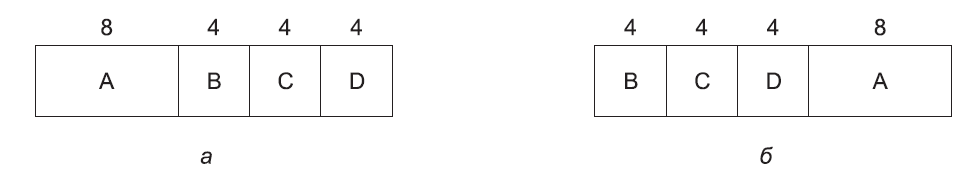
\includegraphics[scale=0.75]{pic4-1.png}
   \caption{Пример планирования, когда первым выполняется самое короткое задание:
      а — запуск четырех заданий в исходном порядке; б — запуск этих заданий в порядке,
      когда самое короткое из них выполняется первым}
\end{figure}

Следует заметить, что алгоритм, основанный на выполнении первым самого короткого
задания, оптимален только в том случае, если все задания доступны одновременно.
В качестве примера противоположной ситуации рассмотрим пять заданий от A до E
со сроками выполнения 2, 4, 1, 1 и 1 соответственно. Время их поступления 0, 0, 3, 3
и 3. Первоначально может быть выбрано только задание A или задание B, а остальные
три задания к тому времени еще не поступят. Используя правило, по которому первым
выполняется самое короткое задание, мы будем выполнять задания в следующей очередности: A, B, C, D, E — при среднем времени ожидания, равном 4,6. Разумеется, их
запуск в следующем порядке: B, C, D, E, A — привел бы к среднему времени ожидания,
равному 4,4.
\newline

\textbf{SRT}

Приоритетной версией алгоритма выполнения первым самого короткого задания
является алгоритм первоочередного выполнения задания с наименьшим оставшимся
временем выполнения. При использовании этого алгоритма планировщик всегда вы-
бирает процесс с самым коротким оставшимся временем выполнения. Здесь, так же
как и прежде, время выполнения заданий нужно знать заранее. При поступлении
нового задания выполняется сравнение общего времени его выполнения с оставши-
мися сроками выполнения текущих процессов. Если для выполнения нового задания
требуется меньше времени, чем для завершения текущего процесса, этот процесс при-
останавливается и запускается новое здание. Эта схема позволяет быстро обслужить
новое короткое задание.
\newpage
%-------------------------------------------------------------------------------------
\subsection{Планирование в интерактивных системах – дисциплины RR, приоритетное планирование}

\textbf{RR}

Модификацией алгоритма FCFS является алгоритм, получивший название Round Robin (Round Robin – это вид детской карусели в США) или сокращенно RR. По сути дела, это тот же самый алгоритм, только реализованный в режиме вытесняющего планирования. Можно представить себе все множество готовых процессов организованным циклически – процессы сидят на карусели. Карусель вращается так, что каждый процесс находится около процессора небольшой фиксированный квант времени, обычно 10 – 100 миллисекунд. Пока процесс находится рядом с процессором, он получает процессор в свое распоряжение и может исполняться.

Каждому процессу назначается определенный интервал времени, называемый его квантом, в течение которого ему предоставляется возможность выполнения. Если процесс к завершению кванта времени все еще выполняется, то ресурс центрального процессора у него отбирается и передается другому процессу. Разумеется, если процесс переходит в заблокированное состояние или завершает свою работу до истечения кванта времени, то переключение центрального процессора на другой процесс происходит именно в этот момент. Алгоритм циклического планирования не представляет сложности в реализации. На
рис. а показано, что от планировщика требуется всего лишь вести список процессов, готовых к выполнению. Когда процесс исчерпает свой квант времени, он, как
показано на рис. б, помещается в конец списка.

\begin{figure}[!h]\center
   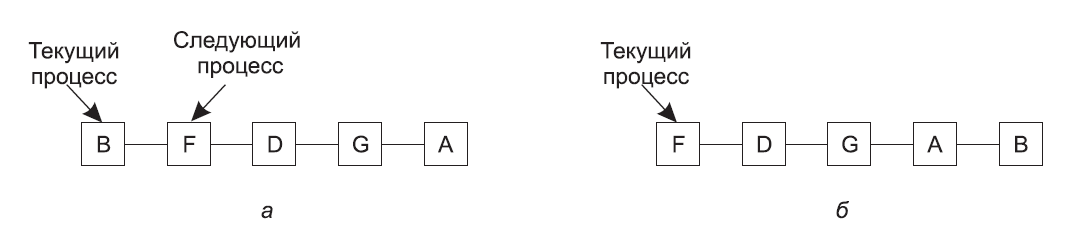
\includegraphics[scale=0.7]{pic4-2.png}
   \caption{Циклическое планирование: а — список процессов, находящихся в состоянии
      готовности; б — тот же список после того, как процесс B исчерпал свой квант времени}
\end{figure}

Единственное, что по-настоящему представляет интерес в циклическом планировании, — это продолжительность кванта времени. Переключение с одного процесса на другой требует определенного количества времени для выполнения задач администрирования — сохранения и загрузки регистров и карт памяти, обновления различных таблиц и списков, сброса на диск и перезагрузки кэша памяти и т. д. Предположим, что переключение процесса, или переключение контекста, как его иногда называют, занимает 1 мс, включая переключение карт памяти, сброс на диск и перезагрузку кэша и т. д. Также предположим, что значение кванта времени установлено на 4 мс. При таких параметрах настройки после 4 мс полезной работы центральному процессору придется затратить (то есть потерять) 1 мс на переключение процесса. Таким образом, 20\% процессорного времени будет выброшено на административные издержки, а это, вне всякого сомнения, слишком много.

Чтобы повысить эффективность использования центрального процессора, мы можем установить значение кванта времени равным, скажем, 100 мс. Теперь теряется всего 1\% времени. Но посмотрим, что получится на серверной системе, если за очень короткое время к ней поступит 50 запросов, имеющих широкий разброс степени востребованности центрального процессора. В список готовых к запуску процессов будет помещено 50 процессов. Если центральный процессор простаивает, первый из них будет запущен немедленно, второй не сможет запуститься, пока не истекут 100 мс, и т. д. Если предположить, что все процессы полностью воспользуются своими квантами времени, то самый невезучий последний процесс может пребывать в ожидании в течение 5 с, прежде чем получит шанс на апуск.Многим пользователям работа системы при пятисекундном ожидании ответа на короткую команду покажется слишком медленной. Эта ситуация получит особо негативную окраску, если некоторые из запросов, размещенные ближе к концу очереди, требуют всего лишь несколько миллисекунд процессорного времени. Если квант времени будет короче, качество их обслуживания улучшится. Другая особенность состоит в том, что если значение кванта времени установлено большим, чем среднее время задействованности центрального процессора, переключение процесса не будет происходить слишком часто. Вместо этого большинство процессов будут выполнять операцию блокировки перед истечением кванта времени, вызывающим переключение процессов. Исключение принудительного прерывания повышает производительность, поскольку переключение процессов происходит только при логической необходимости, то есть когда процесс блокируется и не может продолжить работу. Из этого следует, что установка слишком короткого кванта времени приводит к слишком частым переключениям процессов и снижает эффективность использования центрального процессора, но установка слишком длинного кванта времени может привести к слишком вялой реакции на короткие интерактивные запросы. Зачастую разумным компромиссом считается квант времени в 20–50 мс.

\textbf{Приоритетное планирование}

В циклическом планировании явно прослеживается предположение о равнозначности всех процессов. Зачастую люди, обладающие многопользовательскими компьютерами и работающие на них, имеют на этот счет совершенно иное мнение. К примеру, в университете иерархия приоритетности должна нисходить от декана к факультетам, затем к профессорам, секретарям, техническим работникам, а уже потом к студентам. Необходимость учета внешних факторов приводит к приоритетному планированию. Основная идея проста: каждому процессу присваивается значение приоритетности и запускается тот процесс, который находится в состоянии готовности и имеет наивысший приоритет.

Даже если у персонального компьютера один владелец, на нем могут выполняться несколько процессов разной степени важности. Например, фоновому процессу, отправляющему электронную почту, должен быть назначен более низкий приоритет, чем процессу, воспроизводящему на экране видеофильм в реальном времени. Чтобы предотвратить бесконечное выполнение высокоприоритетных процессов, планировщик должен понижать уровень приоритета текущего выполняемого процесса с каждым сигналом таймера (то есть с каждым его прерыванием). Если это действие приведет к тому, что его приоритет упадет ниже приоритета следующего по этому показателю процесса, произойдет переключение процессов. Можно выбрать и другую альтернативу: каждому процессу может быть выделен максимальный квант допустимого времени выполнения. Когда квант времени будет исчерпан, шанс запуска будет предоставлен другому процессу, имеющему наивысший приоритет.

Приоритеты могут присваиваться процессам в статическом или в динамическом режиме. Например, на военных компьютерах процессы, инициированные генералами, могут начинать свою работу с приоритетом, равным 100, процессы, инициированными полковниками, — с приоритетом, равным 90, майорами — с приоритетом 80, капитанами — 70, лейтенантами — 60 и так далее вниз по табели о рангах. А в коммерческом компьютерном центре высокоприоритетные задания могут стоить 100 долларов в час, задания со средним приоритетом — 75, а задания с низким приоритетом — 50. В UNIX-
системах есть команда nice, позволяющая пользователю добровольно снизить приоритет своего процесса, чтобы угодить другим пользователям, но ею никто никогда не пользуется.

Приоритеты также могут присваиваться системой в динамическом режиме с целью достижения определенных системных задач. К примеру, некоторые процессы испытывают существенные ограничения по скорости работы устройств ввода-вывода и проводят большую часть своего времени в ожидании завершения операций ввода-вывода. Как только такому процессу понадобится центральный процессор, он должен быть предоставлен немедленно, чтобы процесс мог приступить к обработке следующего запроса на ввод-вывод данных, который затем может выполняться параллельно с другим процессом, занятым вычислениями. Если заставить процесс, ограниченный скоростью работы устройств ввода-вывода, долго ждать предоставления центрального процессора, это будет означать, что он занимает оперативную память неоправданно долго. Простой алгоритм успешного обслуживания процессов, ограниченных скоростью работы устройств ввода-вывода, предусматривает установку значения приоритета в 1/f, где f — это часть последнего кванта времени,использованного этим процессом. Процесс, использовавший только 1 мс из отпущенных ему 50 мс кванта времени, должен получить приоритет 50, в то время как процесс, проработавший до блокировки 25 мс, получит приоритет, равный 2, а процесс, использовавший весь квант времени, получит приоритет, равный 1.

Зачастую бывает удобно группировать процессы по классам приоритетности и использовать приоритетное планирование применительно к этим классам, а внутри каждого класса использовать циклическое планирование. На рис. показана система с четырьмя классами приоритетности. Алгоритм планирования выглядит следующим образом: если есть готовые к запуску процессы с классом приоритетности 4, следует запустить каждый из них на один квант времени по принципу циклического планирования, при этом вовсе не беспокоясь о классах с более низким приоритетом. Когда класс с уровнем приоритета 4 опустеет, в циклическом режиме запускаются процессы с классом приоритетности 3. Если опустеют оба класса, 4 и 3, в циклическом режиме запускаются процессы с классом приоритетности 2 и т. д. Если приоритеты каким-то образом не будут уточняться, то все классы с более низким уровнем приоритета могут «умереть голодной смертью».

\begin{figure}[!h]\center
   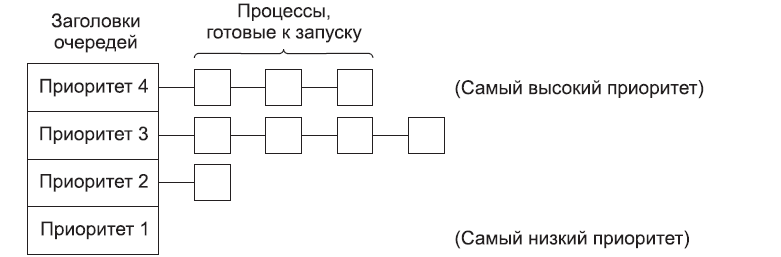
\includegraphics[scale=0.75]{pic4-3.png}
   \caption{Алгоритм планирования для четырех классов приоритетности}
\end{figure}
\newpage
%-------------------------------------------------------------------------------------
\subsection{Планирование в системах реального времени: RMS, EDF}

Системы реального времени относятся к тому разряду систем, в которых время играет
очень важную роль. Обычно одно или несколько физических устройств, не имеющих
отношения к компьютеру, генерируют входные сигналы, а компьютер в определенный
промежуток времени должен соответствующим образом на них реагировать. К примеру, компьютер в проигрывателе компакт-дисков получает биты от привода и должен
превращать их в музыку за очень короткий промежуток времени. Если вычисления
занимают слишком много времени, музыка приобретет довольно странное звучание.
Другими системами реального времени являются система отслеживания параметров
пациента в палате интенсивной терапии, автопилот воздушного судна, устройство
управления промышленными роботами на автоматизированном предприятии. Во всех
этих случаях получение верного результата, но с запозданием, зачастую так же неприемлемо, как и неполучение его вообще.

Системы реального времени обычно делятся на жесткие системы реального времени
(системы жесткого реального времени), в которых соблюдение крайних сроков обяза-
тельно, и гибкие системы реального времени (системы мягкого реального времени),
в которых нерегулярные несоблюдения крайних сроков нежелательны, но вполне
допустимы. В обоих случаях режим реального времени достигается за счет разделе-
ния программы на несколько процессов, поведение каждого из которых вполне предсказуемо и заранее известно. Эти процессы являются, как правило, быстротечными
и способными успешно завершить свою работу за секунду. При обнаружении внешнего
события планировщик должен так спланировать работу процессов, чтобы были со-
блюдены все крайние сроки.

События, на которые должна реагировать система реального времени, могут быть определены как периодические (происходящие регулярно) или апериодические (происходящие непредсказуемо). Возможно, системе придется реагировать на несколько периодических потоковых событий. В зависимости от времени, необходимого на обработку каждого события, с обработкой всех событий система может даже не справиться. Например, если происходит m периодических событий, событие i возникает с периодом Pi и для обработки каждого события требуется Ci секунд процессорного времени, то поступающая  информация может быть обработана только в том случае, если

\begin{figure}[!h]\center
   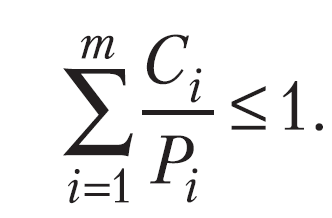
\includegraphics[scale=0.6]{pic4-4.png}
\end{figure}

Система реального времени, отвечающая этому критерию, называется планируемой. Это означает, что такая система фактически может быть реализована. Процесс, не отвечающий этому тесту, не может быть планируемым, поскольку общее время центрального процессора, требуемое процессу, в совокупности больше того времени, которое этот центральный процессор может предоставить. В качестве примера рассмотрим гибкую систему реального времени с тремя периодическими событиями с периодами 100, 200 и 500 мс соответственно. Если на обработку каждого из этих событий требуется, соответственно, 50, 30 и 100 мс процессорного времени, работа системы может быть спланирована, поскольку 0,5 + 0,15 + 0,2 < 1.
Если будет добавлено четвертое событие с периодом 1 с, то система будет сохранять
планируемость до тех пор, пока на обработку этого события не потребуется более
150 мс процессорного времени. В этом вычислении подразумевается, что издержки на
переключение контекста настолько малы, что ими можно пренебречь.
Алгоритмы планирования работы систем реального времени могут быть статическими или динамическими. Первый из них предусматривает принятие решений по
планированию еще до запуска системы, а второй — их принятие в реальном времени,
после того как начнется выполнение программы. Статическое планирование работает только при условии предварительного обладания достоверной информацией
о выполняемой работе и о крайних сроках, которые нужно соблюсти. Алгоритмы
динамического планирования подобных ограничений не имеют.

\textbf{Общее планирование реального времени}

Используется модель, когда каждый процесс борется за процессор со своим заданием и графиком его выполнения.
Планировщик должен знать:
\begin{itemize}
   \item частоту, с которой должен работать каждый процесс
   \item объем работ, который ему предстоит выполнить
   \item ближайший срок выполнения очередной порции задания
\end{itemize}

Рассмотрим пример из трех процессов.
\begin{itemize}
   \item Процесс А запускается каждые 30мс, обработка кадра 10мс
   \item Процесс В частота 25 кадров, т.е. каждые 40мс, обработка кадра 15мс
   \item Процесс С частота 20 кадров, т.е. каждые 50мс, обработка кадра 5мс
\end{itemize}

\begin{figure}[!h]\center
   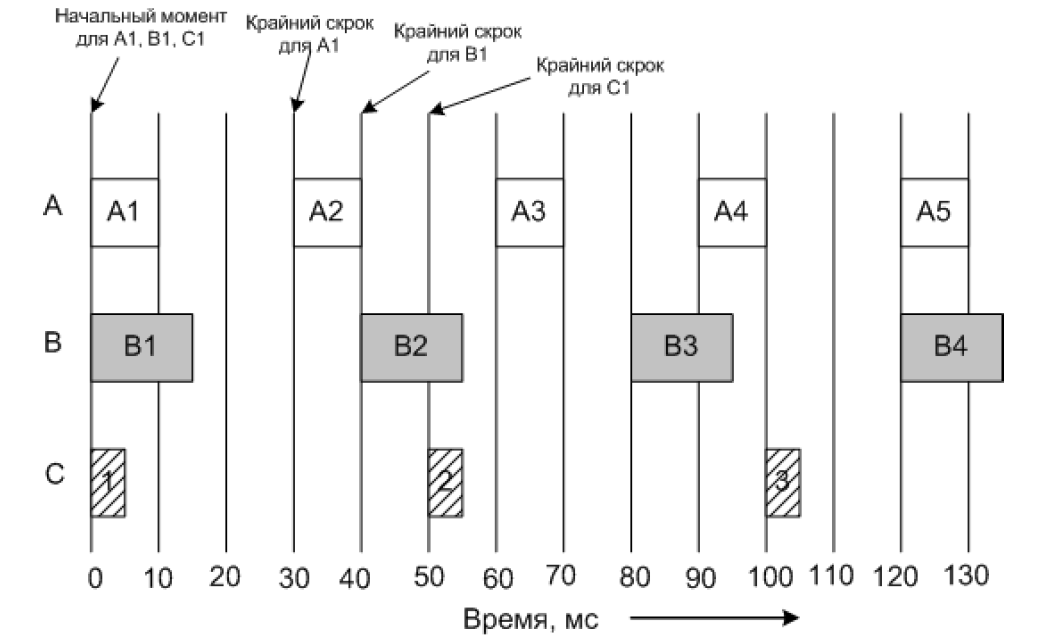
\includegraphics[scale=0.7]{pic4-5.png}
   \caption{Три периодических процесса}
\end{figure}

10/30+15/40+5/50=0.808<1

Условие выполняется, планировать можно.
Будем планировать эти процессы статическим(приоритет заранее назначается каждому процессу) и динамическим методами.

\textbf{Статический алгоритм планирования RMS (Rate Monotonic Scheduling)}

Процессы должны удовлетворять условиям:

\begin{itemize}
   \item  Процесс должен быть завершен за время его периода
   \item  Один процесс не должен зависеть от другого
   \item  Каждому процессу требуется одинаковое процессорное время на каждом интервале
   \item  У непериодических процессов нет жестких сроков
   \item  Прерывание процесса происходит мгновенно
\end{itemize}

Приоритет в этом алгоритме пропорционален частоте.
Процессу А он равен 33 (частота кадров)
Процессу В он равен 25
Процессу С он равен 20
Процессы выполняются по приоритету.

\begin{figure}[!h]\center
   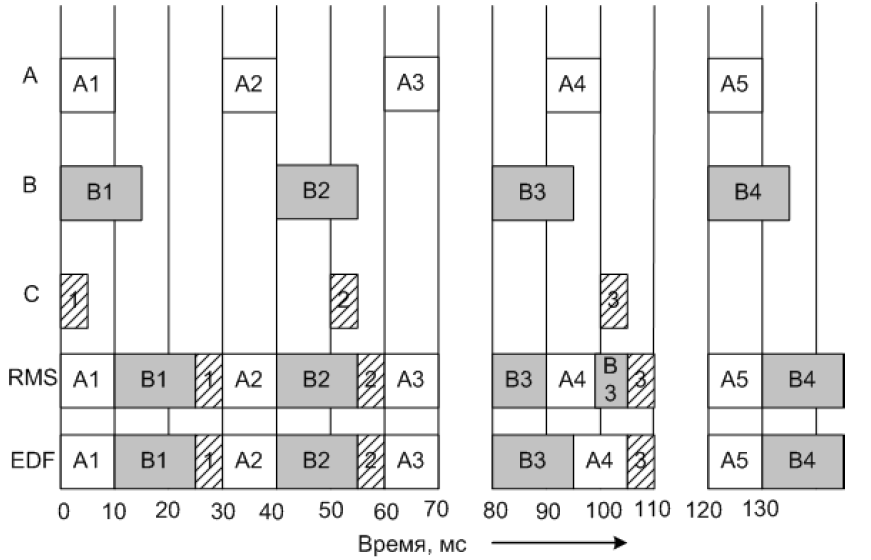
\includegraphics[scale=0.7]{pic4-6.png}
   \caption{Статический алгоритм планирования RMS (Rate Monotonic Scheduling)}
\end{figure}
\newpage

\textbf{Динамический алгоритм планирования EDF (Earliest Deadline First)}

Наибольший приоритет выставляется процессу, у которого осталось наименьшее время выполнения.

При больших загрузках системы EDF имеет преимущества.
Рассмотрим пример, когда процессу А требуется для обработки кадра - 15мс.
Проверяем, можно ли планировать эти процессы.

15/30+15/40+5/50=0.975<1

Загрузка системы 97.5\%

\begin{figure}[!h]\center
   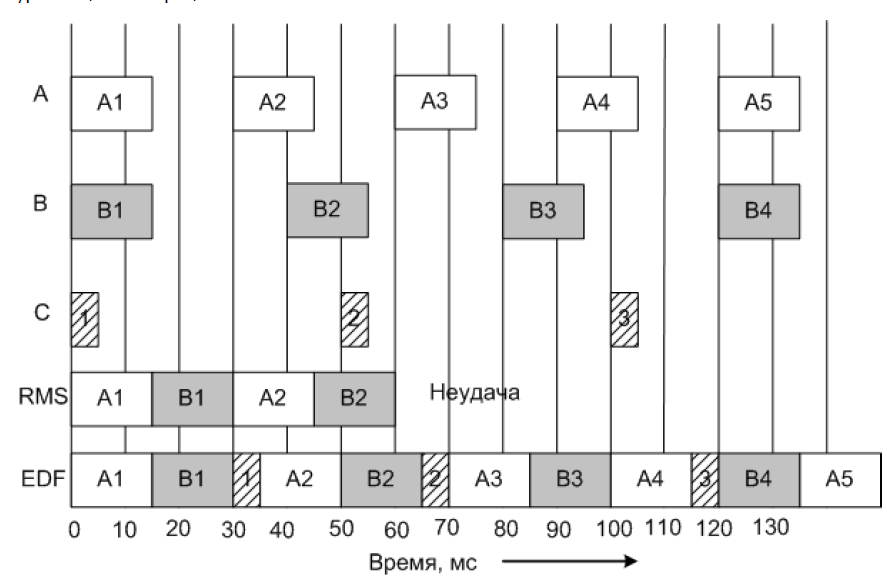
\includegraphics[scale=0.7]{pic4-7.png}
   \caption{Динамический алгоритм планирования EDF (Earliest Deadline First)
      Алгоритм планирования RMS терпит неудачу.}
\end{figure}


%------------------------------------------------------------------------------------
